%%%%%%%% ICML 2026 EXAMPLE LATEX SUBMISSION FILE %%%%%%%%%%%%%%%%%

\documentclass{article}

\usepackage[UTF8,fontset=none,heading=false]{ctex}
\setCJKmainfont[AutoFakeBold=2.5,ItalicFont={Songti SC}]{Songti SC}
\setCJKsansfont[AutoFakeBold=2.5]{Hiragino Sans GB}
\setCJKmonofont[Scale=0.92]{Hiragino Sans GB}
\XeTeXlinebreaklocale "zh"
\XeTeXlinebreakskip = 0pt plus 1pt

% Recommended, but optional, packages for figures and better typesetting:
\usepackage{microtype}
\usepackage{graphicx}
\usepackage{enumitem}
\usepackage{subcaption}
\usepackage{booktabs} % for professional tables

% hyperref makes hyperlinks in the resulting PDF.
% If your build breaks (sometimes temporarily if a hyperlink spans a page)
% please comment out the following usepackage line and replace
% \usepackage{icml2026} with \usepackage[nohyperref]{icml2026} above.
\usepackage{hyperref}


% Attempt to make hyperref and algorithmic work together better:
\newcommand{\theHalgorithm}{\arabic{algorithm}}

% Use the following line for the initial blind version submitted for review:
\usepackage[preprint]{icml2026_zh}
\setmainfont{texgyretermes-regular.otf}[
  BoldFont=texgyretermes-bold.otf,
  ItalicFont=texgyretermes-italic.otf,
  BoldItalicFont=texgyretermes-bolditalic.otf
]
\setsansfont{texgyreheros-regular.otf}[
  BoldFont=texgyreheros-bold.otf,
  ItalicFont=texgyreheros-italic.otf,
  BoldItalicFont=texgyreheros-bolditalic.otf
]
\setmonofont{texgyrecursor-regular.otf}[
  BoldFont=texgyrecursor-bold.otf,
  ItalicFont=texgyrecursor-italic.otf,
  BoldItalicFont=texgyrecursor-bolditalic.otf,
  Scale=MatchLowercase
]
\renewcommand{\figurename}{图}
\renewcommand{\tablename}{表}
\captionsetup[figure]{name=图}
\captionsetup[table]{name=表}
\renewcommand{\refname}{参考文献}
\renewcommand{\appendixname}{附录}

% For preprint, use
% \usepackage[preprint]{icml2026}

% If accepted, instead use the following line for the camera-ready submission:
% \usepackage[accepted]{icml2026}

\usepackage{amsmath}
\usepackage{amssymb}
\usepackage{mathtools}
\usepackage{booktabs}
\usepackage{threeparttable}
\usepackage{graphicx}
\usepackage{amsthm}
\usepackage{multirow}
\usepackage[table]{xcolor}
\usepackage{xspace}
\usepackage{makecell}   
\usepackage[frozencache,cachedir=minted-cache-zh]{minted}
% \usepackage[finalizecache,cachedir=minted-cache]{minted}
\usepackage{listings}
\usepackage[most]{tcolorbox}
\tcbuselibrary{listingsutf8}
\usepackage{booktabs} 
\usepackage{threeparttable}
% \usepackage{algorithm}
% \usepackage{algpseudocode}
% Customize
\newcommand{\red}[1]{\textcolor{red}{#1}\xspace}

\definecolor{rowgray}{gray}{0.85}
\definecolor{rowlightblue}{RGB}{215, 230, 255} 

\newcommand{\hlfirst}[1]{\colorbox[HTML]{CFE2FF}{#1}}  % 深一点（模拟不透明）
\newcommand{\hlsecond}[1]{\colorbox[HTML]{E8F1FF}{#1}} % 浅一点（模拟半透明）
\newcommand{\blue}[1]{\textcolor{blue}{#1}\xspace}

% if you use cleveref..
\usepackage[capitalize,noabbrev]{cleveref}

%%%%%%%%%%%%%%%%%%%%%%%%%%%%%%%%
% THEOREMS
%%%%%%%%%%%%%%%%%%%%%%%%%%%%%%%%
\theoremstyle{plain}
\newtheorem{theorem}{Theorem}[section]
\newtheorem{proposition}[theorem]{Proposition}
\newtheorem{lemma}[theorem]{Lemma}
\newtheorem{corollary}[theorem]{Corollary}
\theoremstyle{definition}
\newtheorem{definition}[theorem]{Definition}
\newtheorem{assumption}[theorem]{Assumption}
\theoremstyle{remark}
\newtheorem{remark}[theorem]{Remark}
\definecolor{gemblue}{RGB}{225, 240, 255}
% Todonotes is useful during development; simply uncomment the next line
%    and comment out the line below the next line to turn off comments
%\usepackage[disable,textsize=tiny]{todonotes}
\usepackage[textsize=tiny]{todonotes}

% The \icmltitle you define below is probably too long as a header.
% Therefore, a short form for the running title is supplied here:
\icmltitlerunning{\textsc{AOrchestra}}

\newcommand{\our}{\textsc{AOrchestra}\xspace}

\begin{document}

\twocolumn[
  \icmltitle{\textsc{AOrchestra}：面向智能体编排的子智能体自动创建}

  \begin{icmlauthorlist}
      \icmlauthor{Jianhao Ruan\textsuperscript{*}}{1,3}
      \icmlauthor{Zhihao Xu\textsuperscript{*}}{2}
      \icmlauthor{Yiran Peng}{1}
      \icmlauthor{Fashen Ren}{3}
      \icmlauthor{Zhaoyang Yu}{1} \\
      \icmlauthor{Xinbing Liang}{4}
      \icmlauthor{Jinyu Xiang}{3}
      \icmlauthor{Yongru Chen}{3}
      \icmlauthor{Bang Liu}{5}
      \icmlauthor{Chenglin Wu}{1}
      \icmlauthor{Yuyu Luo}{3}
      \icmlauthor{Jiayi Zhang}{1,3}
    \end{icmlauthorlist}



\icmlaffiliation{1}{DeepWisdom}
\icmlaffiliation{2}{中国人民大学}
\icmlaffiliation{3}{香港科技大学（广州）}
\icmlaffiliation{4}{华东师范大学}
\icmlaffiliation{5}{蒙特利尔大学与 Mila}

  \icmlcorrespondingauthor{Yuyu Luo}{yuyuluo@hkust-gz.edu.cn}
  \icmlcorrespondingauthor{Jiayi Zhang}{jzhang361@connect.hkust-gz.edu.cn}
  \vskip 0.3in
]

% this must go after the closing bracket ] following \twocolumn[ ...

% This command actually creates the footnote in the first column listing the
% affiliations and the copyright notice. The command takes one argument, which
% is text to display at the start of the footnote. The \icmlEqualContribution
% command is standard text for equal contribution. Remove it (just {}) if you
% do not need this facility.

% Use ONE of the following lines. DO NOT remove the command.
% If you have no special notice, KEEP empty braces:
\printAffiliationsAndNotice{}  % no special notice (required even if empty)
% Or, if applicable, use the standard equal contribution text:
% \printAffiliationsAndNotice{\icmlEqualContribution}


\begin{abstract}
语言智能体在任务自动化方面展现出巨大潜力。随着任务变得日益复杂且执行周期更长，为充分发挥这种潜力，面向多轮任务求解的“子智能体即工具”范式逐渐兴起。然而，现有设计仍缺少对子智能体的\emph{动态抽象}视角，因而适应性不足。为应对这一挑战，我们提出一种统一且与框架无关的智能体抽象，将任意智能体表示为四元组 $\langle Instruction, Context, Tools, Model \rangle$。该四元组可视作能力的组合配方，使系统能够按任务需要创建专用执行器。在此基础上，我们提出智能体系统 \textsc{AOrchestra}。其中央编排器会在每一步实例化该四元组：筛选与任务相关的上下文，选择工具和模型，并通过即时自动创建智能体来委派执行。这一设计能够减少人工工程投入，同时保持框架无关性，并以即插即用的方式支持多种智能体作为任务执行器。它还支持可控的性能与成本权衡，使系统能够逼近帕累托有效前沿。在三个具有挑战性的基准（GAIA、SWE-Bench 和 Terminal-Bench）上，与 Gemini-3-Flash 搭配时，\textsc{AOrchestra} 相比最强基线取得了 $16.28\%$ 的相对提升。代码地址：\url{https://github.com/FoundationAgents/AOrchestra}
\end{abstract}

% \input{files/1-introduction}
\section{引言}
人类依靠集体智慧与协作能力处理复杂的长程工作~\cite{gao2025evolvesurvey,DBLP:journals/corr/abs-2510-23587,DBLP:journals/corr/abs-2510-17586}。如今，智能体也在不断迈向类似的复杂多轮任务~\cite{yao2024tau, zhang2025autoenv, xu2026unlocking}，因此，设计良好的智能体系统已成为突破单一模型性能上限的重要途径~\cite{liu2025advances}。

\begin{figure}[t!]
    \centering
    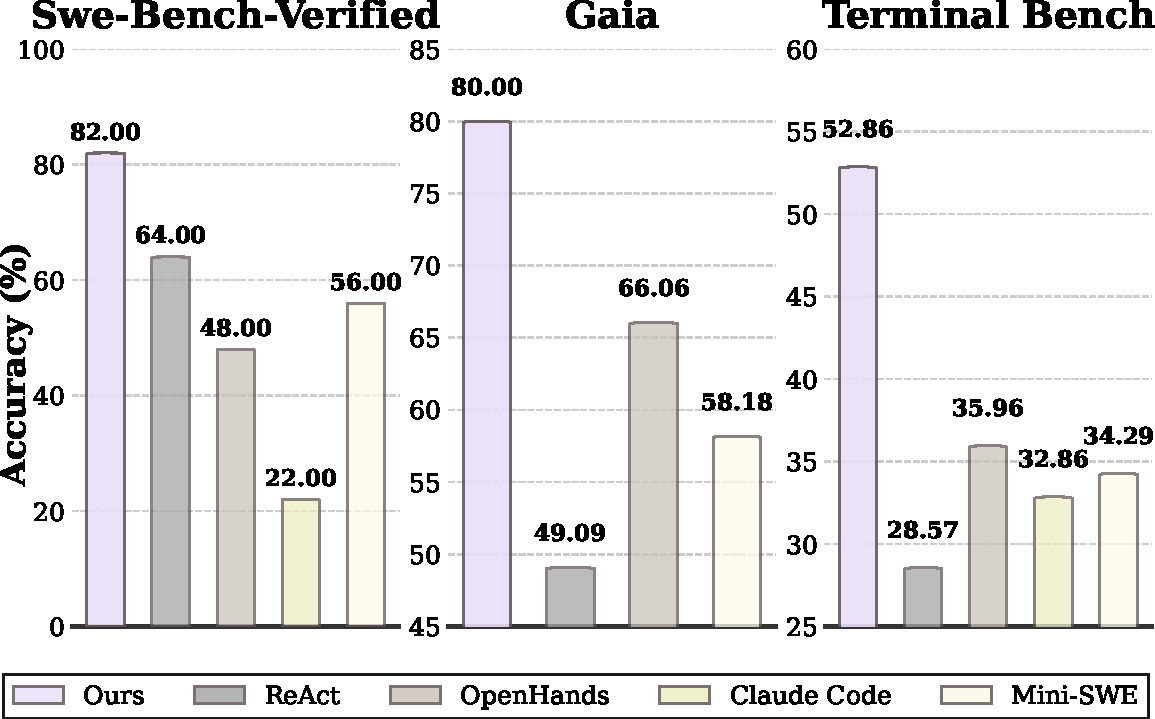
\includegraphics[width=\linewidth]{figures/abs.pdf}
    \caption{在 Gemini-3-Flash 配置下，\our 与其他常用智能体框架在三个高难度智能体基准（GAIA、Terminal-Bench 2.0 和 SWE-Bench-Verified）上的整体性能对比。}
    \label{fig:performance}
\end{figure}

为应对日益复杂的应用场景，早期工作通常依赖固定的协作流程或多智能体系统~\cite{hong2023metagpt, hu2025owl, DBLP:journals/corr/abs-2510-17586}。多智能体协作虽然有助于任务分解，但在开放式环境中往往带来显著的协调开销，且难以精细控制上下文路由，容易出现含噪信息过度共享或关键信息被遗漏的问题，从而使稳健的长程执行变得困难~\cite{gao2025single}。

\begin{figure*}[htbp]
    \centering
    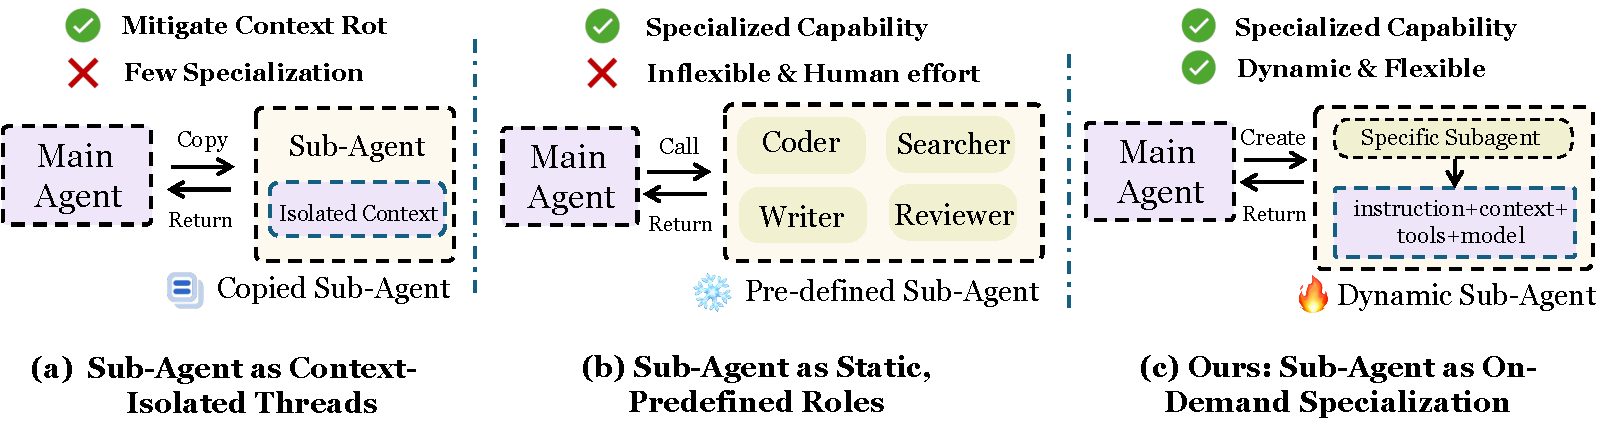
\includegraphics[width=\linewidth]{figures/diff.pdf}
    \caption{“子智能体即工具”方法对比。\textbf{(a) 将子智能体视为上下文隔离线程}可以缓解上下文退化，却无法按需专门化。\textbf{(b) 将子智能体视为静态角色}能够提供专用能力，但缺乏灵活性，存在能力覆盖空缺，并需要大量人工工程。\textbf{(c) 我们的按需专门化子智能体}通过实例化统一四元组抽象 \textsc{(Instruction, Context, Tools, Model)}，即时创建针对具体任务定制的执行器。}
    \label{fig:diff}
\end{figure*}

因此，较新的方法逐渐转向更实用的“子智能体即工具”范式：主智能体（即编排器）通过显式工具调用，将任务委派给子智能体。然而，现有设计在实践中仍缺乏灵活性，并经常退化为图~\ref{fig:diff} 所示的两种受限模式：
(1) \textit{将子智能体视为上下文隔离线程。}THREAD~\cite{schroeder2025thread} 和 Context-Folding~\cite{sun2025scaling} 等系统主要把子智能体视为彼此隔离的上下文线程，以避免上下文退化~\citep{hong2025context}。但现实任务中的子任务往往需要专门能力，因此这类系统无法充分发挥专用子智能体的潜力。
(2) \textit{将子智能体视为静态角色。}Claude Code~\cite{anthropic_claude_code_subagents} 和 Chain-of-Agents~\cite{li2025chain} 等系统将每个子智能体设定为静态角色，其能力与协作模式通常被硬编码。预先定义的一组子智能体无法覆盖开放环境中动态出现的各类子任务，而且高度依赖人工工程，难以适配不同环境。

本文提出 \our{}，一个面向复杂长程任务的智能体框架。我们的核心观点是从\textbf{按需专门化}的角度看待子智能体，如图~\ref{fig:diff}(c) 所示。我们认为，子智能体应被视为灵活的抽象单元，而不是预定义的固定角色。系统由此可以在运行时动态组合能力，根据具体任务需要实例化定制的子智能体。
具体而言，\emph{任意}智能体都可以通过统一四元组 \textsc{(instruction, context, tools, model)} 描述为可实例化单元。专门化围绕智能体求解任务所需的两个互补维度展开：(1) \emph{工作记忆（instruction, context）}，即智能体必须达成的目标，以及作出判断时应依据的证据。尤其是，context 属性只注入与当前子任务最相关的信息，从而过滤可能造成干扰的细节。(2) \emph{能力（tools, model）}，即为达成目标，智能体被赋予哪些可执行能力。系统按子任务组合特定工具与模型，使每个子智能体都具备精确且任务专用的功能。二者共同使系统能够为每项任务自动创建专用子智能体。

基于这一按需专门化视角，我们进一步引入专用编排器。它直接操作四元组接口，动态自动创建定制子智能体。编排器本身不执行任务，只负责系统编排：将总体目标动态分解为下一项子任务，通过显式工具调用创建专门化的定制子智能体，并将执行工作委派给它。
这种解耦设计具有多项优势。第一，动态创建机制可以让每个子智能体拥有独特能力和干净的工作上下文，显著提高任务执行准确率。第二，编排器不依赖子智能体的内部实现，因此子智能体可以完全即插即用。第三，编排器可以从交互经验中训练或学习，其能力范围既包括创建智能体的基础技能，也包括自适应模型选择等高级特性，从而在成本与性能之间取得更优平衡。

大量实验表明，\our{} 在开放世界环境中具有更强的性能和更广泛的泛化能力。我们首先在免训练设置下，对三个高难度智能体基准进行评测：Terminal-Bench 2.0~\cite{tbench_2025}（Bash 环境）、SWE-Bench~\cite{jimenez2023swe}（编程环境）和 GAIA~\cite{mialon2023gaia}（数字世界环境）。如图~\ref{fig:performance} 所示，我们的方法在所有基准上均持续优于具有代表性的子智能体编排方法~\cite{anthropic_claude_code_subagents}和广泛使用的智能体框架~\cite{wang2024openhands, yang2024sweagent}。尤其是在搭配 \texttt{Gemini3-Flash} 时，我们的框架取得了 $16.28\%$ 的提升，验证了该编排模型在复杂长程任务中的优越性。

更重要的是，\our 自然支持从经验中学习编排策略。我们通过两种方式实例化这一能力：(1) 使用监督微调提升编排器的子任务分解与四元组合成能力，使 GAIA 上的编排质量提升 $11.51\%$ pass@1；(2) 使用上下文学习优化成本感知路由，使 GAIA pass@1 提升 $3.03\%$，同时将平均成本降低 $18.5\%$，得到更优的成本与性能帕累托前沿。

总体而言，我们的贡献如下：
\begin{itemize}
    \item 我们提出 \our，一个以编排器为中心的智能体系统。它通过统一四元组接口 \textsc{(Instruction, Context, Tools, Model)}，将子智能体视为可\emph{动态创建}的执行器，从而以任务充分的上下文和显式能力控制实现按需专门化。
    \item \our 在 Terminal-Bench 2.0、SWE-Bench-Verified 和 GAIA 上取得了强劲的免训练性能，并持续优于常用智能体系统。与 Gemini-3-Flash 搭配时，相比最强基线取得了 $16.28\%$ 的相对提升。
    \item 我们从两个互补角度表明该设计下的编排策略是可学习的：监督微调可以提升基础任务编排能力（$+11.51\%$），通过上下文学习实现的成本感知路由则带来更优的成本与性能帕累托权衡（平均成本降低 $18.5\%$）。
\end{itemize}

\section{相关工作}
\paragraph{多智能体系统}
受协作式问题求解的启发，早期研究提出多智能体系统（MAS）以增强语言模型的任务求解能力~\cite{zhang2025agentorchestra, DBLP:journals/corr/abs-2505-07437,wu2024autogen, shi2025aime, gao2025single, zhu2025oagents, fang2025cognitive, zhang2024aflow,DBLP:conf/icml/Li0FXC0L25}。例如，MetaGPT~\cite{hong2023metagpt} 将智能体组织为结构化的软件开发工作流，由产品经理、架构师等专门角色通过预定义通信协议协作。OWL~\cite{hu2025owl} 采用规划器与工作器工作流，将领域无关的规划和领域相关的执行模块化，以改善迁移与泛化。尽管这类方法有效，大多数多智能体系统通常依赖固定工作流，因此较为僵化。AutoAgents~\cite{chen2023autoagents} 虽然提出为不同任务构建不同的多智能体系统，但完成任务时仍然依赖固定工作流。这促使研究逐渐转向\emph{子智能体即工具}范式，下一部分将介绍相关工作~\cite{gao2025evolvesurvey, gao2025single}。\our{} 也遵循这一范式，并进一步强调以编排为中心、动态创建子智能体，而不依赖特定的人工设计工作流。

\paragraph{子智能体即工具}
这类方法由主智能体模型以类似工具调用的方式调用子智能体来解决问题~\cite{li2025chain, su2025toolorchestra, grand2025self,DBLP:journals/tkde/LiuSLMJZFLTL25}。例如，THREAD~\cite{schroeder2025thread} 可以递归创建子智能体来处理分解后的子问题。类似地，Context-Folding~\cite{sun2025scaling} 针对子任务创建分支，再将中间步骤压缩为简洁摘要并折叠回主上下文，以此管理上下文。然而，这些方法没有把子智能体视为完全专门化的智能体，因而未能充分利用它们。Claude Code~\cite{anthropic_claude_code_subagents} 等实用系统支持在隔离上下文窗口中运行、具有自定义系统提示与工具权限的子智能体，但这些子智能体通常仍被配置为固定专家，需要人工设计。\our{} 将每个子智能体视为动态单元，并提出一种以编排为中心的智能体系统，主动按需动态创建这类子智能体，从而解决上述局限。

% \input{files/3-methods}
\section{方法}

本节首先在第~\ref{sec:formulation} 节形式化问题，随后在第~\ref{sec:method_design} 节详细介绍 \our 的设计，最后在第~\ref{sec:learnable} 节说明专用编排器的训练过程。图~\ref{fig:piepine} 给出了方法概览。

\begin{figure*}[t]
    \centering
    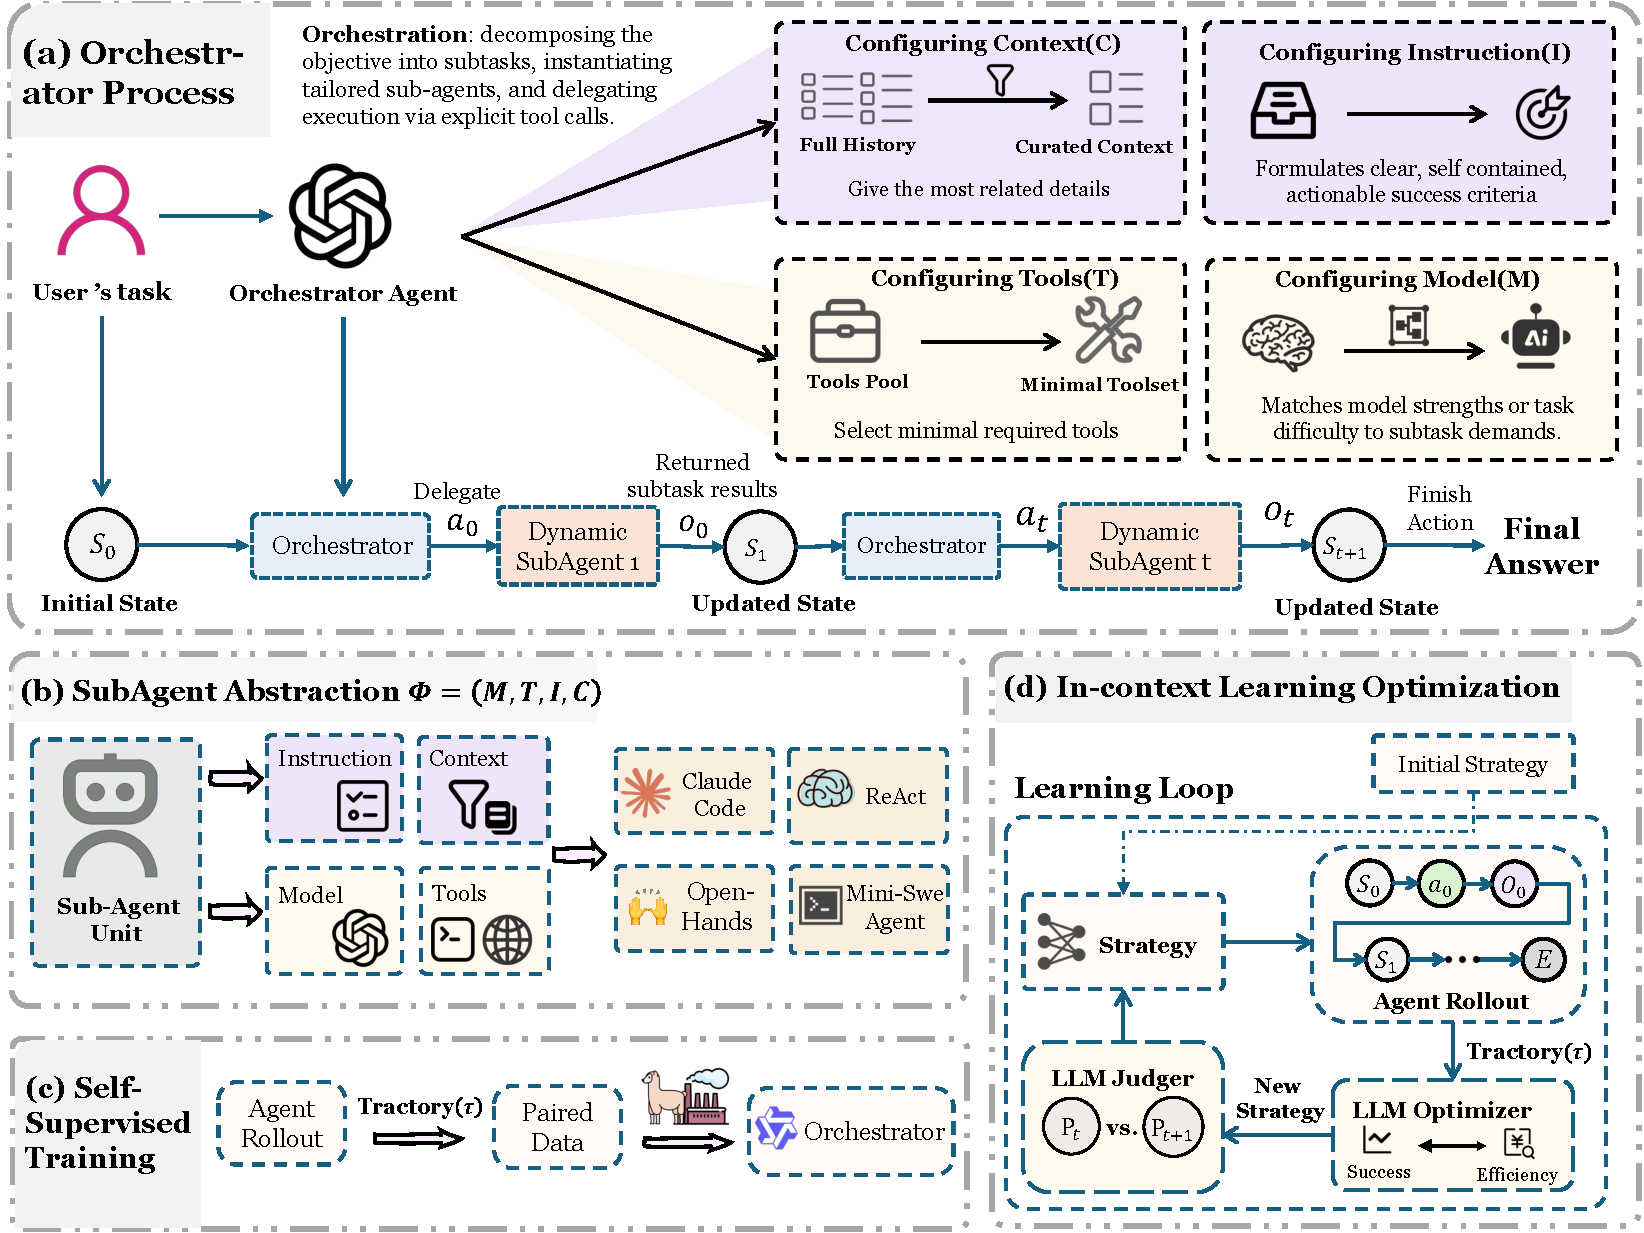
\includegraphics[width=\textwidth]{figures/introduction.pdf}
    \caption{面向复杂长程任务的智能体框架 \our{} 总体设计。编排器通过反复将子任务委派给即时实例化的子智能体来完成用户任务，每个子智能体都由统一四元组 $(I,C,T,M)$ 定义。编排器本身可学习，并能从以往经验中改进任务分解、上下文路由和能力分配。}
    \label{fig:piepine}
\end{figure*}

\subsection{问题形式化}
\label{sec:formulation}
本文主要关注复杂智能体任务。智能体系统通过与环境进行多步交互来完成用户目标 $G$。环境提供\emph{环境级}动作空间 $\mathcal{A}_{\text{env}}$，例如 shell 命令、网页操作和代码编辑，并返回观测、工具输出和错误消息等反馈。因此，一项任务的交互轨迹可定义为：
\[
\tau = (s_0, a_0, o_0, s_1, a_1, o_1, \dots, s_T),
\]
其中，$s_t \in \mathcal{S}$ 表示第 $t$ 步的系统状态，包括累积历史、中间结果与环境反馈；$a_t$ 表示第 $t$ 步采取的动作；$o_t \in \mathcal{O}$ 表示返回的观测。系统按照如下状态转移函数演化：
\[
s_{t+1} = \delta(s_t, a_t, o_t),
\]
其中，$\delta: \mathcal{S} \times \mathcal{A}_{\text{env}} \times \mathcal{O} \rightarrow \mathcal{S}$ 将当前状态、动作和观测映射到下一状态，即把新返回的信息纳入系统内部状态。

\paragraph{子智能体即工具视角。}
我们关注“子智能体即工具”范式。在该范式中，\emph{主智能体}（编排器）既可以直接在环境中行动，也可以通过工具调用把子任务委派给子智能体。相应地，编排器操作一个\emph{系统级}动作空间，通常包含三类动作：(1) 环境动作 $u \in \mathcal{A}_{\text{env}}$；(2) 调用子智能体执行的委派动作（\texttt{Delegate}$(\cdot)$）；(3) 终止动作（\texttt{Finish}）。我们将这一通用编排动作空间记为：
\[
\mathcal{A}_{\text{orch}} \supseteq \mathcal{A}_{\text{env}} \ \cup\ \{\texttt{Delegate}(\cdot),\ \texttt{Finish}(y)\}.
\]
不同系统的主要差异在于如何参数化 \texttt{Delegate}，例如只携带上下文进行委派，或委派给一组固定角色；另一项差异是编排器本身是否也执行环境动作。

我们的目标是最大化任务成功率，并可选择性地权衡执行成本：
\[
\max_{\pi}\ \mathbb{E}\Big[\mathbf{1}\{\text{Success}(G)\}-\lambda\cdot \text{Cost}(\tau)\Big],
\]
其中，$\pi$ 是编排器策略，$\text{Cost}(\tau)$ 可以包括 token 用量、工具调用次数、延迟或货币成本，$\lambda$ 控制成本与性能之间的权衡。

\subsection{\our{}}
\label{sec:method_design}

\paragraph{统一的四元组智能体抽象。}
\our{} 使用统一且与框架无关的抽象对\emph{主智能体和子智能体}建模。我们把一个智能体实例定义为可实例化的四元组：
\[
\Phi = (I, C, T, M),
\]
其中，$I$ 是规定当前目标与成功标准的任务指令；$C$ 是经过筛选、供智能体作出判断的工作上下文；$T$ 是定义智能体动作空间的工具集合；$M$ 是与环境交互的底层模型。该抽象显式分离了两个需要\textit{专门化}的互补维度：\emph{工作记忆} $(I,C)$ 与\emph{能力} $(T,M)$。需要强调的是，我们不把子智能体视为静态实体，而是将其视为可在运行时参数化和创建的\emph{动态}单元。

主智能体（编排器）同样可以表示为四元组 $\Phi^{\text{main}}=(I^{\text{main}},C^{\text{main}},T^{\text{main}},M^{\text{main}})$。区别在于，$T^{\text{main}}$ 提供的是用于编排的\emph{系统工具}，如 \texttt{Delegate} 和 \texttt{Finish}，而不是 $\mathcal{A}_{\text{env}}$ 中的环境工具。

\paragraph{编排器的动作空间。}
基于上述抽象，\our{} 将编排与执行解耦。\our{} 的编排器从不直接执行 $\mathcal{A}_{\text{env}}$ 中的环境动作，而只操作以下两种动作：
\[
\mathcal{A}_{\our} = \{\texttt{Delegate}(\Phi),\ \texttt{Finish}(y)\}.
\]
在第 $t$ 步，编排器采样动作 $a_t \in \mathcal{A}_{\our}$。若 $a_t=\texttt{Delegate}(\Phi_t)$，系统会创建执行器 $A(\Phi_t)$ 来执行子任务并返回观测 $o_t$；若 $a_t=\texttt{Finish}(y)$，交互以最终答案 $y$ 终止。返回的观测通过 $s_{t+1}=\delta(s_t,a_t,o_t)$ 纳入下一状态。

\paragraph{\texttt{Delegate} 与 \texttt{Finish} 的实现。}
我们为 \our{} 的编排器提供两个系统工具：\texttt{Delegate} 和 \texttt{Finish}。\texttt{Delegate} 接收 $\Phi_t=(I_t,C_t,T_t,M_t)$ 作为参数，并据此实例化执行器。该执行器使用模型 $M_t$，只能访问工具集合 $T_t$，且仅以 $(I_t,C_t)$ 为条件执行任务。它向编排器返回结构化观测 $o_t$，通常包括：(1) 简洁的结果摘要；(2) 相关产物，如文件和参考资料；(3) 执行失败时的错误消息或日志。\texttt{Finish} 终止交互并输出最终响应 $y$。

\paragraph{\our{} 的优势。}
我们提出的 \our{} 具有多项关键优势。第一，它会按需为每个子智能体动态配备定制能力，显著提高任务执行准确率。与以往工作~\cite{sun2025scaling, anthropic_claude_code_subagents} 不同，编排器会有意识地向子智能体提供结构良好的上下文。第~\ref{sec:adv1} 节将表明，这种谨慎的上下文管理可以增强模型求解任务的能力。第二，编排器只操作四元组抽象，不依赖子智能体的内部实现。因此，我们可以采用多种子智能体设计，例如简单的 ReAct 方法~\cite{yao2022react} 或 mini-SWE 智能体。第三，编排器可以从大量经验中学习。第~\ref{sec:learnable} 节将进一步说明，这些可学习能力既包括基础任务编排技能，即做什么、依据哪些信息以及使用哪些工具，也包括自适应模型路由等高级能力，其目标可以是通过选择最合适的模型来平衡性能与成本。

\subsection{可学习的编排器}
\label{sec:learnable}

在 $\mathcal{A}_{\our}=\{\texttt{Delegate}(\Phi),\texttt{Finish}(y)\}$ 下，编排任务可以表述为学习结构化动作上的策略：
\[
\pi_\theta(a_t \mid s_t),\quad a_t\in\mathcal{A}_{\our}.
\]

由于委派参数 $\Phi_t=(I_t,C_t,T_t,M_t)$ 是显式可用的，学习可聚焦于两个互补维度：(1) \textbf{任务编排}，决定做什么、使用哪些上下文以及采用哪些工具；(2) \textbf{模型路由}，选择 $M_t$，即要调用的模型，以平衡性能与成本。下面分别介绍这两种学习范式。

\paragraph{用于任务编排的监督微调（SFT）。}
给定专家编排轨迹 $\{(s_t,a_t^\star)\}$，我们通过行为克隆微调编排器：
\[
\theta^\star = \arg\max_{\theta}\ \sum_{t} \log p_{\theta}(a_t^\star \mid s_t),
\]
其中，$a_t^\star$ 是专家动作，可以是 $\texttt{Delegate}(\Phi_t^\star)$ 或 $\texttt{Finish}(y^\star)$。在我们的设置中，SFT 主要蒸馏\emph{任务编排}能力：改善子任务分解与 $(I_t,C_t,T_t)$ 的合成，从而为每一步生成更好的工作记忆和更合适的工具子集。本文优先展示训练专用编排器的潜力，因此采用直接的 SFT 方法。其他工作也可以使用 GRPO~\cite{shao2024deepseekmath} 等训练方法来增强任务编排能力。

\paragraph{用于成本感知编排的迭代式上下文内学习。}
除更新参数外，我们还可以通过迭代交互学习编排器的\emph{指令}（提示词），在不改变模型权重的情况下优化编排。具体而言，我们把编排器指令 $I^{\text{main}}$ 作为可学习对象，在环境中运行 \our{}，收集轨迹 $\tau=\{(s_t,a_t,o_t)\}_{t=0}^{T}$ 以及任务性能和执行成本等结果指标。随后，优化模型分析这些轨迹，并提出提示词修改 $\Delta I$ 来更新指令：
\[
I^{\text{main}}_{k+1} = \textsc{Optimize}\bigl(I^{\text{main}}_{k},\ \tau_k,\ \text{Perf}(\tau_k),\ \text{Cost}(\tau_k)\bigr),
\]
其中，$k$ 表示优化轮次。系统在环境中使用更新后的编排器反复执行 $N$ 轮，以改进成本感知的编排行为，例如模型选择、路由决策和工具使用模式，并寻找性能与成本之间的帕累托有效权衡。

\section{实验}

\subsection{实验设置}

\begin{table*}[!t]
\centering
\small
\setlength{\tabcolsep}{5pt}
\renewcommand{\arraystretch}{1.1}
\begin{threeparttable}
\caption{在不同模型下，\our 与基线智能体系统在 GAIA、Terminal-Bench 2.0 和 SWE-Bench-Verified 上的对比。最佳结果以\textbf{粗体}标出。}
\label{tab:main_results}
\begin{tabular}{l l cc cc cc c}
\toprule
\textbf{方法} & \textbf{模型配置}
& \multicolumn{2}{c}{\textbf{GAIA}}
& \multicolumn{2}{c}{\textbf{Terminal-Bench 2.0}}
& \multicolumn{2}{c}{\textbf{SWE-Bench-Verified}}
\\
\cmidrule(lr){3-4}\cmidrule(lr){5-6}\cmidrule(lr){7-8}
&
& \textbf{Pass@1} & \textbf{Pass@3}
& \textbf{Pass@1} & \textbf{Pass@3}
& \textbf{Pass@1} & \textbf{Pass@3}
& \textbf{平均 Pass@1}\\
\midrule

\multirow[c]{3}{*}{ReAct}
& Gemini-3-Flash     & 49.09 & 66.06 & 28.57 & 47.14 & 64.00 & 82.00 & 47.22 \\
& DeepSeek-V3.2      & 46.70 & 71.51 & 20.00 & 32.86 & 48.00 & 87.00 & 38.23 \\
& Claude-4.5-haiku   & 47.88 & 62.42 & 20.00 & 37.14 & 63.00 & 87.00 & 43.62 \\
\cmidrule(lr){1-9}

\multirow[c]{3}{*}{OpenHands}
& Gemini-3-Flash     & 66.06 & 72.73 & 31.43 & 51.43 & 48.00 & 66.00 & 48.49 \\
& DeepSeek-V3.2      & 63.64 & 72.12 & 21.43 & 35.71 & 60.00 & 75.00 & 48.35 \\
& Claude-4.5-haiku   & 54.55 & 61.21 & 12.85 & 25.71 & 68.00 & 83.00 & 45.13 \\
\cmidrule(lr){1-9}

\multirow[c]{3}{*}{Mini-SWE}
& Gemini-3-Flash     & 58.18 & 68.48 & 34.29 & 50.00 & 56.00 & 85.00 & 49.49 \\
& DeepSeek-V3.2      & 50.30 & 63.63 & 30.00 & 48.57 & \textbf{84.00} & \textbf{89.00} & 54.76 \\
& Claude-4.5-haiku   & 40.61 & 60.00 & 24.29 & 28.57 & 44.00 & 83.00 & 36.30 \\
\cmidrule(lr){1-9}

\multirow[c]{2}{*}{Claude Code}
& Gemini-3-Flash     & -- & -- & 32.86 & 48.57 & 22.00 & 42.00 & 27.43 \\
& Claude-4.5-haiku   & -- & -- & 34.29  & 45.71 & 25.00 & 41.00 & 29.65 \\
\midrule

\multirow[c]{3}{*}{\our}
& Gemini-3-Flash     & \textbf{80.00} & \textbf{86.06} & \textbf{52.86} & \textbf{57.14} & 82.00 & 86.00 & \textbf{71.62} \\
& DeepSeek-V3.2      & 67.87 & 80.00 & 31.43 & 42.86 & 76.00 & 82.00 & 58.43 \\
& Claude-4.5-haiku   & 60.61 & 73.90 & 35.71 & 45.71 & 70.00 & 84.00 & 55.44 \\
\bottomrule
\end{tabular}
\end{threeparttable}
\end{table*}

\textbf{基准。}我们在三个具有挑战性的智能体基准上评测所提出的方法，它们覆盖不同的交互环境：(1) \textbf{Terminal-Bench 2.0}~\cite{tbench_2025}，它将智能体置于带有交互式 Bash shell 的 Linux 终端中，要求执行命令行操作来完成多步现实任务；(2) \textbf{SWE-Bench-Verified}~\cite{jimenez2023swe}，它在真实 GitHub 项目上评估软件工程能力，要求智能体在真实编程环境中定位缺陷、实现补丁并通过给定测试套件；(3) \textbf{GAIA}~\cite{mialon2023gaia} 验证集，这是一个通用基准，用于测试智能体解决需要多步推理和工具使用的现实任务的能力。我们分别报告所有基准上的 pass@1 和 pass@3。附录~\ref{app:dataset} 进一步说明这些数据集的评测用法，附录~\ref{app:action_space} 则介绍每个基准所使用的工具。

\textbf{模型与基线。}
我们将所提出的方法与以下代表性框架比较：(1) \textbf{ReAct}~\cite{yao2022react}，一个直接基于 ReAct 构建、交替执行推理与动作的简单单智能体系统；(2) \textbf{OpenHands}~\cite{wang2024openhands}，一个常用于解决多类现实任务的开放智能体平台；(3) \textbf{mini-SWE-agent}~\cite{yang2024sweagent}，一个面向 GitHub issue 等任务的精简编程智能体；(4) \textbf{Claude Code}~\cite{anthropic_claude_code_subagents}，一个生产级智能体命令行工具，支持创建预定义子智能体以分解任务并隔离上下文。对于每个智能体系统，我们使用三个前沿语言模型，包括两个强模型 \texttt{Gemini-3-Flash} 和 \texttt{DeepSeek-V3.2}~\cite{liu2025deepseek}，以及一个较小模型 \texttt{Claude-4.5-haiku}。基线实现详见附录~\ref{app:baseline_imp}。

\textbf{实现。}
所有实验中，编排器的 $max\_attempt$ 设为 10，子智能体的 $max\_step$ 设为 50。为保证公平比较，所有基线的 $max\_step$ 均设为 500。免训练设置的设计详见附录~\ref{app:prompt_used}，其中给出了三个基准中使用的全部编排器和子智能体提示词。子智能体完成任务后，由一个评审 LLM 检查执行轨迹并总结核心信息。

对于 SFT 训练，我们在非思考模式下微调 Qwen3-8B~\cite{yang2025qwen3}，以增强其编排能力。我们使用 TaskCraft~\cite{shi2025taskcraft} 作为种子数据集，并用 Gemini-3-Flash 收集 2K 条编排轨迹进行 SFT 训练。SFT 阶段使用 LLaMAFactory 框架~\cite{zheng2024llamafactory} 进行 2 个 epoch 的全参数微调，学习率为 1e-5。更多细节见附录~\ref{app:sft_hyper}。

对于上下文内学习，我们使用 \texttt{Claude Sonnet 4.5} 作为优化模型，迭代更新编排器指令。实验执行 5 轮优化，每轮收集 6 条交互轨迹用于分析。每轮结束后，选取成本与性能权衡最优的提示词，即以更低成本获得最高性能的提示词，作为下一轮的初始化。

\subsection{主要结果}
\label{sec:main_results}
表~\ref{tab:main_results} 给出了 \our 与基线智能体系统在 GAIA、Terminal-Bench 2.0 和 SWE-Bench-Verified 三个基准上的主要结果，评测指标为 pass@1/pass@3。对于 \our，我们使用 \texttt{Gemini-3-Flash} 作为编排器；为便于比较，此处只提供一个模型作为子智能体选项。总体来看，\our 在所有环境中均持续优于基线。使用 \texttt{Gemini-3-Flash} 时，\our{} 在三个基准上的平均 pass@1 比最佳基线高 $22.13\%$。

\paragraph{GAIA 结果。}
GAIA 衡量通用智能体解决现实任务的能力，包括多跳搜索、文件处理和多模态操作。在这一环境中，\our 相比所有基线取得了最佳性能。具体而言，当编排器和子智能体均使用 \texttt{Gemini-3-Flash} 时，\our 的 pass@1 为 80.00，pass@3 为 86.06，优于所有基线。在相同的 \texttt{Gemini-3-Flash} 主干模型下，\our 将 pass@1 从最强基线框架 \texttt{OpenHands} 的 66.06 提升至 80.00，绝对提高 13.94 个百分点。即使使用能力较弱的 \texttt{Claude-4.5-haiku} 作为子智能体模型，它在 GAIA 上仍达到 60.61 pass@1，说明性能提升并不局限于能力最强的模型配置。由于 Claude Code 被设计为生产级编程智能体，我们未在 GAIA 上评测它，因此相应结果留空。GAIA 案例研究见附录~\ref{app:case_study}。

\paragraph{Terminal-Bench 2.0 结果。}
Terminal-Bench 评估智能体在受现实工作流启发的计算机终端环境中的操作能力。在该基准上，采用 \texttt{Gemini-3-Flash} 的 \our 取得 52.86 pass@1 和 57.14 pass@3。与表~\ref{tab:main_results} 中 pass@1 为 34.29 的最强基线 \texttt{Mini-SWE} 相比，pass@1 绝对提升 64.29 个百分点。除 \texttt{Gemini-3-Flash} 配置外，\our 在其他主干模型下仍具竞争力，其性能与 \texttt{Claude Code} 等专用编程智能体系统相当或更好。

\paragraph{SWE-Bench-Verified 结果。}
SWE-Bench-Verified 通过要求智能体为开源仓库中的真实问题生成能够通过给定测试的代码补丁，评估其解决实际问题的能力。在该基准上，\our 在不同主干模型下均表现强劲，并可与最优基线系统竞争。使用 \texttt{Gemini-3-Flash} 时，\our 达到 82.00 pass@1 和 86.00 pass@3，优于相同模型设置下的 \texttt{ReAct} 和 \texttt{OpenHands}。与专门面向软件任务的 \texttt{Mini-SWE} 相比，\our 仍具竞争力，并且在三个模型主干上均稳定达到超过 70.00 的 pass@1。

\subsection{\our 的优势分析}
\label{subsec:adv}
本节分析 \our 动态创建专用子智能体的优势，重点关注工作记忆与能力。总体而言，我们发现，由编排器向子智能体显式传递上下文能够提升性能（第~\ref{sec:adv1} 节）；针对不同任务选择不同模型可以获得成本与性能的帕累托权衡（第~\ref{sec:adv2} 节）；多种子智能体实现也能持续改善整体性能（第~\ref{sec:adv3} 节）。

\subsubsection{优势一：上下文共享}
\label{sec:adv1}

\begin{table}[t]
\centering
\small
\setlength{\tabcolsep}{6pt}
\renewcommand{\arraystretch}{1.15}
\caption{调用子智能体时的上下文控制消融。各设置仅改变传给子智能体的 \texttt{Context} 字段，以隔离上下文继承的影响；子智能体模型、工具和系统提示均保持一致。}
\label{tab:context_control}
\begin{tabular}{l c c c c}
\toprule
\textbf{设置} & \textbf{Level 1} & \textbf{Level 2} & \textbf{Level 3} & \textbf{平均值} \\
\midrule
无上下文    & 89.47 & 81.48 & 75.00 & 86.00 \\
完整上下文  & 94.74 & 77.78 & 75.00 & 84.00 \\
\textbf{本文方法} & \textbf{100.00} & \textbf{88.89} & \textbf{75.00} & \textbf{96.00} \\
\bottomrule
\end{tabular}
\end{table}

在 \our{} 中，编排器会向每个新创建的子智能体显式、动态地传递筛选后的上下文。为评估该设计的有效性，我们将其与两个变体比较：\textbf{无上下文}，每个子智能体只接收任务指令；\textbf{完整上下文}，每个子智能体继承主智能体的全部上下文。这两种方法也常见于以往系统~\cite{sun2025scaling, anthropic_claude_code_subagents}。我们在 GAIA 上开展分析，从验证集中抽取 50 个样本。

表~\ref{tab:context_control} 表明，有必要将上下文视为子智能体的重要组成部分，并把它抽象为四元组中的一个元素。具体而言，无上下文设置由于缺失关键执行轨迹和前序步骤中的细粒度线索而失败；完整上下文设置则经常引入无关信息，加剧上下文退化。相比之下，我们的方法允许编排器只选择和压缩与任务相关的历史，从而提供更干净的上下文并取得最高分。

\subsubsection{优势二：可学习的编排器}
\label{sec:adv2}

\begin{table}[htbp]
\centering
\small
\setlength{\tabcolsep}{8pt}
\caption{主要结果。ReAct 每次运行只使用一个指定语言模型，其他系统则可以使用单模型或混合模型池。ICL 表示上下文内学习。}
\label{tab:level_main}
\resizebox{\linewidth}{!}{%
\begin{tabular}{l l c c}
\toprule
\textbf{系统} & \textbf{语言模型} & \textbf{准确率} & \textbf{平均成本} \\
\midrule

\multirow{5}{*}{ReAct}
& Claude-4.5-sonnet  & 53.93 & 0.190 \\
& Claude-4.5-haiku   & 47.88 & 0.066 \\
& Gemini-3-Flash     & 49.09 & 0.070 \\
& GPT-5-mini         & 54.55 & 0.052 \\
& Deepseek-v3.2      & 46.70 & 0.027 \\
\midrule

\multirow{4}{*}{Ours}
& Gemini-3-Flash     & \textbf{80.00} & 0.79 \\
& Claude-4.5-sonnet  & 71.52 & 0.91 \\
& GPT-5-mini         & 67.27 & 0.28 \\
& Deepseek-v3.2      & 67.87 & 0.14 \\
\midrule
Ours (Gemini-3-Flash) & Mixed & 72.12 & 0.70 \\
Ours (ICL)   & Mixed &\textbf{75.15} & \textbf{0.57} \\
\midrule
Ours (Qwen3-8B) & Gemini-3-Flash & 56.97 & 0.36 \\
Ours (SFT) & Gemini-3-Flash & \textbf{68.48} & \textbf{0.68} \\
\bottomrule
\end{tabular}
}
\end{table}

\paragraph{用于任务编排的监督微调（SFT）。}
\our{} 的一个现实考量是，编排质量取决于主智能体分解目标和生成高质量委派四元组的能力。为研究这种敏感性，我们将主智能体替换为能力较弱的 \texttt{Qwen3-8B}，同时保持 \texttt{Gemini-3-Flash} 作为子智能体执行器。如表~\ref{tab:level_main} 所示，该设置（\textsc{Ours (Qwen3-8B)}）以平均成本 \$0.36 达到 $56.97\%$ 的准确率。虽然低于使用强主智能体的配置（采用 \texttt{Gemini-3-Flash} 的 \textsc{Ours} 达到 $80.00\%$），但仍超过使用 \texttt{Gemini-3-Flash} 的 ReAct。这一差距说明，即便只使用较弱的 8B 模型，编排仍然有效。随后，我们通过 SFT 微调 \texttt{Qwen3-8B} 的编排能力，使准确率从 $56.97\%$ 大幅提升至 $68.48\%$（表~\ref{tab:level_main}），代价是每项任务的平均成本增加 \$0.32。执行轨迹分析表明，微调后的模型在处理复杂任务时表现出更强的长程问题求解能力，总尝试次数相比基础模型增加 $56\%$。这一增益说明，编排是一种可有效改善的可学习技能。

\begin{figure}[]
    \centering
    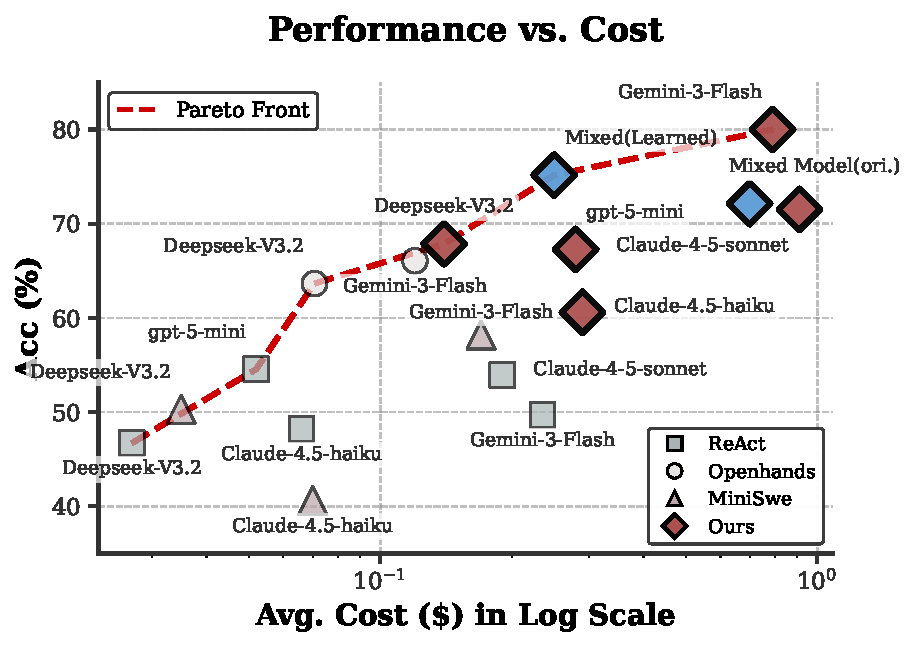
\includegraphics[width=\linewidth]{figures/gaia_cost_performance.pdf}
    \caption{\textbf{GAIA 的帕累托前沿曲线。}图中绘制 GAIA 准确率和每项任务的平均成本（美元，对数刻度）。每个点对应一种配置，虚线表示 \our 在不同模型路由选择下形成的帕累托前沿。}
    \label{fig:cost}
\end{figure}

\paragraph{用于成本感知编排的上下文内学习。}
\our{} 的另一项优势是能够通过逐步模型路由平衡成本与性能。表~\ref{tab:level_main} 表明，使用不同子智能体模型会形成明显不同的准确率与成本曲线，因此编排器必须感知这种权衡。为此，我们采用面向帕累托前沿的上下文学习过程，根据带有性能与货币成本反馈的交互轨迹，迭代优化编排器指令。得到的策略在降低成本的同时改进了 \our：在混合模型设置中，Ours (ICL) 将准确率从 $72.12\%$ 提升至 $75.15\%$，同时把平均成本从 \$0.70 降至 \$0.57（表~\ref{tab:level_main}），说明简单的提示词级学习能够同时提高性能与效率。在系统层面，图~\ref{fig:cost} 进一步表明 \our 可以自然形成帕累托有效的运行点：在不同模型选择下，我们的配置构成帕累托前沿，相比基线系统性地改善了成本与性能的权衡。

\subsubsection{优势三：即插即用的子智能体}
\label{sec:adv3}
本节验证该方法在框架层面的可插拔性。具体而言，我们在 Terminal-Bench 上使用 \texttt{Gemini-3-Flash} 作为编排器，并按照附录~\ref{app:dataset} 的设置，将子智能体的执行后端替换为 ReAct 风格、Mini-SWE 风格等不同智能体框架。

表~\ref{tab:plugin_subagent} 表明，当使用不同的子智能体后端时，\our 仍能保持稳定性能，并持续优于相应基线。该设计使子智能体可以充当即插即用的模块，让系统无需依赖任何特定子智能体实现也能保持稳健。

\begin{table}[]
\centering
\setlength{\tabcolsep}{6pt}
\caption{在固定编排器下评估即插即用的子智能体。我们使用 Gemini-3-Flash 测试不同子智能体实现的稳健性与可复用性。}
\label{tab:plugin_subagent}
\resizebox{\linewidth}{!}{%
\begin{tabular}{l c c c c}
\toprule
\textbf{系统}
& \textbf{简单}
& \textbf{中等}
& \textbf{困难}
& \textbf{准确率} \\
\midrule
\multicolumn{5}{l}{\textbf{独立基线}} \\
\midrule
ReAct                     & 50.00 & 34.09 & 16.67 & 28.57 \\
Mini-SWE-Agent            & 50.00 & 40.91 & 20.83 & 34.29 \\
Claude Code               & 50.00 & 41.86 & 16.67 & 32.86 \\
\midrule
\multicolumn{5}{l}{\textbf{带可插拔子智能体的编排器}} \\
\midrule
ReAct 风格子智能体       & 50.00 & \textbf{63.63} & 20.83 & \textbf{48.57} \\
Mini-SWE 风格子智能体    & \textbf{100.00} & 47.73 & \textbf{33.33} & 44.29 \\
\bottomrule
\end{tabular}
}
\end{table}

\section{结论}
本文提出 \our{}，一个以编排为中心的智能体系统。它通过统一四元组接口（Instruction、Context、Tools、Model）自动创建子智能体，以解决复杂长程智能体任务。通过将子智能体视为可动态创建的单元，编排器能够按需生成针对任务定制的执行器，并为其提供专用工作记忆（指令、上下文）和能力（模型、工具）。

这一抽象具有现实价值：它以任务充分的上下文支持按需专门化，并使不同实现下的子智能体保持即插即用。抽象与执行的解耦使编排器具备可学习性；我们给出了两种优化方式，即监督微调与上下文学习。实验结果表明，当搭配 Gemini-3-Flash 等前沿模型时，\our{} 在三个高难度基准（GAIA、Terminal-Bench 和 SWE-Bench-Verified）上均取得强劲且稳定的提升。它显著优于已有基线框架，例如在所有基准上的 pass@1 平均提高 16.28 个百分点。这些结果验证了以编排为中心的方法在自动处理复杂长程任务时的有效性。




% \input{files/7-statement}
\bibliography{cited}
\bibliographystyle{icml2026}

% files/6-appendix.tex

\clearpage
\onecolumn
\appendix
% \section{Appendix}
\label{sec:appendix}

%%%%%%%%%%%%%%%%%%%%%%%%%%%%%%%%%%%%%%%%%%%%%%%%%%%%%%%%%%%%
\section{实现细节}
\label{app:A}

%-----------------------------------------------------------
\subsection{数据集}
\label{app:dataset}
\begin{itemize}
    \item \textbf{GAIA}~\cite{mialon2023gaia}: 
    GAIA 通过真实且需要工具辅助的问题评测通用 AI 助手，这些问题通常涉及网页浏览和多步推理。我们在包含 165 项任务的 GAIA 验证集上评测 \our{}，并将其与其他基线比较。

    \item \textbf{Terminal Bench 2.0}~\cite{tbench_2025}：Terminal-Bench 在沙箱化命令行环境中，以可执行测试为评分依据，评估智能体完成端到端现实工作流的能力。我们在共包含 89 项任务的 Terminal-Bench 2.0 测试集上评测 \our{} 并与其他基线比较。考虑到成本，主要实验随机抽取其中 70 项任务。

    \item \textbf{SWE-Bench-Verified:}~\cite{jimenez2023swe} 
    SWE-Bench Verified 要求智能体生成补丁来解决真实仓库中的真实 GitHub issue，并通过运行测试进行验证，以此衡量自主软件工程能力。Verified 划分经过人工筛查，移除了存在问题的样例。我们在共包含 500 项任务的 SWE-Bench Verified 测试集上评测 \our{} 并与其他基线比较。考虑到成本，我们随机抽取 100 项任务进行评测。
\end{itemize}

\subsection{SFT 超参数}
\label{app:sft_hyper}
实验采用表~\ref{tab:hyper_sft_qwen} 所列的超参数。

\begin{table}[htbp]
\centering
\resizebox{0.5\textwidth}{!}{
\begin{tabular}{l|c|l|c|}
\hline
\textbf{超参数} & \textbf{取值} & \textbf{超参数} & \textbf{取值} \\ \hline
学习率        & 1e-5            & 权重衰减         & 0.05            \\
预热比例      & 0.1             & 最大长度         & 16K            \\
学习率调度器  & cosine          & 批大小           & 64              \\
epoch         & 2               & BF16             & True            \\
DeepSpeed     & zero3           & 工具调用模板     & Hermes          \\ \hline
\end{tabular}
}
\caption{实验所用的 SFT 超参数。}
\label{tab:hyper_sft_qwen}
\end{table}


%-----------------------------------------------------------
\subsection{基线实现}
\label{app:baseline_imp}
在基线实现方面，我们评测了多种广泛使用的智能体框架。实验发现，由于架构与预期使用方式的限制，\texttt{Claude Code} 并不适合 GAIA 的开放世界多跳问答，因此主要实验未报告 \texttt{Claude Code} 的相应结果。

此外，根据初步调查和实证测试，我们发现 \texttt{DeepSeek-V3.2} 与 \textsc{Claude Code} 的原生兼容性较差，因此表~\ref{tab:main_results} 未包含该实验。

在 Terminal-Bench 和 SWE-Bench 评测中，我们使用 \texttt{Harbor} 脚手架，在统一执行接口下运行 \texttt{MiniSWE}、\texttt{OpenHands} 和 \texttt{Claude Code}。


%%%%%%%%%%%%%%%%%%%%%%%%%%%%%%%%%%%%%%%%%%%%%%%%%%%%%%%%%%%%
\section{提示词}
\label{app:prompt_used}

%-----------------------------------------------------------
\subsection{主智能体提示词}
\label{app:B1}

\subsubsection{GAIA 主智能体提示词}
\label{app:B1_gaia}
% TODO: paste GAIA Main Agent prompt (tcolorbox + minted{text})

\begin{tcolorbox}[title={\textbf{\small GAIA 主智能体提示词}}, boxrule=1pt, arc=0mm, colback=black!5!white, colframe=black!75!white, breakable, before skip=10pt, after skip=10pt, pad at break=2mm, parbox=false]

\begin{minted}[fontsize=\scriptsize, breaklines=breakanywhere, frame=lines, framesep=2mm, tabsize=4, style=vs, autogobble]{python}
"""
[GAIA 基准 - 问答任务]
你是 MainAgent（编排器）。你的任务是把给定问题分解为若干子任务，
将每个子任务委派给一个子智能体，从而解决该问题。

决策过程：
1. 检查下方的子任务历史，核对每次尝试的状态、结果和关键发现
2. 评估：现有结果是否足以回答问题？
   - 若任一子任务返回了状态为 "done" 的有效结果 -> 考虑使用 'complete'
   - 若子任务状态为 "incomplete" -> 查看其关键发现，判断已经完成了什么
3. 决定下一步动作：
   - 结果充分 -> 使用 'complete' 并给出答案
   - 仍需工作 -> 对剩余工作使用 'delegate_task'（不要重复已经完成的内容）

预算意识：
- 你的尝试次数有限（见下方进度）
- 每次委派都会消耗时间和资源，请根据任务复杂度合理选择模型
- 若结果看起来正确且已经验证，请相信该结果并完成任务

==== 模型选择指南 ====
{model_pricing_table}

模型选择策略：
- 简单任务选择成本较低的模型
- 复杂推理或关键尝试选择能力更强的模型

==== 进度 ====
[尝试 {attempt_index}/{max_attempts}] 剩余 {remaining_attempts} 次
预算有限，请让每次尝试都发挥作用。

==== 问题 ====
{instruction}

==== 子任务历史 ====
{subtask_history if subtask_history else "尚未完成任何子任务。"}

==== 可用工具 ====
{tools_description}


==== 输出 ====
答案格式：GAIA 要求答案准确、简洁（单个词、数字或短语）。
不要在 answer 字段中加入解释。

返回 JSON：

若结果充分：
{{
  "action": "complete",
  "reasoning": "子任务结果表明 [X]，足以回答该问题",
  "params": {{ "answer": "简洁答案" }}
}}

若仍需进一步工作：
{{
  "action": "delegate_task", 
  "reasoning": "此前尝试已得到 [X]，但仍需 [Y] 才能回答问题",
  "params": {{
    "task_instruction": "一个具体、可执行的子任务
    （例如：'提取论文 2211.xxxxx 摘要中的第二个词'）",
    "context": "此前尝试得到的相关发现",
    "model": "{sub_models} 中的一个",
    "tools": ["GoogleSearchAction", "ExtractUrlContentAction", 
    "ExecuteCodeAction", "ImageAnalysisAction", "ParseAudioAction"]
  }}
}}
"""
\end{minted}
\end{tcolorbox}



\subsubsection{Terminal-Bench 主智能体提示词}
\label{app:B1_terminal}
% TODO: paste Terminal-Bench Main Agent prompt (tcolorbox + minted{text})

\begin{tcolorbox}[title={\textbf{\small Terminal-Bench 主智能体提示词}}, boxrule=1pt, arc=0mm, colback=black!5!white, colframe=black!75!white, breakable, before skip=10pt, after skip=10pt, pad at break=2mm, parbox=false]
\begin{minted}[fontsize=\scriptsize, breaklines=breakanywhere, frame=lines, framesep=2mm, tabsize=4, style=vs, autogobble]{python}

"""
你是 MainAgent（编排器）。你的任务是通过向 SubAgent 委派工作，
完成给定的软件安装或配置任务。

关键事项：容器生命周期
- 每个 SubAgent 都在一个全新容器中运行；若再次执行 delegate_task，先前工作将丢失
- 当 SubAgent 报告 status="done" 时，立即使用 'submit' 在该容器中运行测试

==== 决策过程 ====
1. 仔细阅读原始任务，识别全部要求和边界情况
2. 检查子任务历史，核对状态和已完成步骤
3. 根据任务要求核验 SubAgent 的工作：
   - SubAgent 是否测试了任务提到的全部要求？
   - SubAgent 是否测试了边界情况？（例如，任务若提到 "keyboard interrupt"，是否实际测试过？）
   - SubAgent 标记为 "completed" 的项目是否确实满足任务要求？
4. 决策：
   - status="done" 且核验通过 -> 使用 'submit'
   - status="done" 但核验发现部分要求未满足 -> 使用 'delegate_task' 修复
   - status="partial" -> 使用 'delegate_task'，并在上下文中说明成功和失败的内容

{budget_warning}

==== 模型选择 ====
{model_pricing_table}

==== 进度 ====
[尝试 {attempt_index}/{max_attempts}] 剩余 {remaining_attempts} 次

==== 任务 ====
{instruction}

==== 子任务历史 ====
{subtask_history if subtask_history else "尚未完成任何子任务。"}

==== 可用工具 ====
{tools_description}

==== 输出 ====
返回 JSON：

若 SubAgent 的 status="done"，且你已确认所有任务要求均已满足：
{{
  "action": "submit",
  "reasoning": "核验完成：[列出已满足的任务要求]。正在提交。",
  "params": {{ "reason": "任务完成：[与任务要求对应的具体成果]" }}
}}

若 SubAgent 的 status="done"，但核验发现缺漏：
{{
  "action": "delegate_task",
  "reasoning": "SubAgent 声称已完成，但存在[具体缺漏]：任务要求 [X]，SubAgent 只测试了 [Y]",
  "params": {{
    "task_instruction": "关键：此前尝试遗漏了[具体要求]。
                        你必须：[准确的修复步骤]",
    "context": " 此前 SubAgent 声称完成但遗漏：[具体缺漏]\\n-
                 有效步骤：[应保留的步骤]\\n-
                 必须修复：[遗漏内容]",
    "model": "{sub_models} 中的一个"
  }}
}}

若 SubAgent 的 status="partial"：
{{
  "action": "delegate_task",
  "reasoning": "SubAgent 已取得部分进展，需要继续完成[剩余工作]",
  "params": {{
    "task_instruction": "从此前 SubAgent 停下的位置继续：[具体后续步骤]",
    "context": "根据子任务历史：\\n-
                 有效步骤：[需要重复的步骤]\\n-
                 失败尝试：[需要避免的方法]",
    "model": "{sub_models} 中的一个"
  }}
}}
"""
\end{minted}
\end{tcolorbox}



\subsubsection{SWE-Bench 主智能体提示词}
\label{app:B1_swe}
% TODO: paste SWE-Bench Main Agent prompt (tcolorbox + minted{text})

\begin{tcolorbox}[title={\textbf{\small SWE-Bench 主智能体提示词}}, boxrule=1pt, arc=0mm, colback=black!5!white, colframe=black!75!white, breakable, before skip=10pt, after skip=10pt, pad at break=2mm, parbox=false]
\begin{minted}[fontsize=\scriptsize, breaklines=breakanywhere, frame=lines, framesep=2mm, tabsize=4, style=vs, autogobble]{python}

"""你是 SWE-Bench 任务的 MainAgent（编排器）。
你的目标是通过向 SubAgent 委派工作来修复一个 GitHub issue。


==== 任务 ====
{instruction}

仓库：{repo}
实例：{instance_id}

==== 决策过程 ====
1. 仔细阅读任务，理解 GitHub issue 及需要修复的内容
2. 检查子任务历史，核对 SubAgent 的进度、已完成步骤和测试结果
3. 根据任务要求进行核验：
   - SubAgent 是否定位了有缺陷的代码？
   - SubAgent 是否作出了适当的代码修改？
   - SubAgent 是否运行测试并确认修复有效？
4. 决策：
   - status="done" 且测试通过 -> 使用 'submit'
   - status="done" 但测试失败或不完整 -> 使用 'delegate_task' 修复剩余问题
   - status="partial" -> 使用 'delegate_task' 并提供后续步骤指导

关键事项：SWE-Bench 容器行为
- 当 SubAgent 报告 status="done" 且测试通过时，使用 'submit' 触发最终评测
- 'submit' 会运行官方测试套件（FAIL_TO_PASS + PASS_TO_PASS 测试）以判定是否成功


==== 模型选择 ====
{model_pricing_table}

==== 进度 ====
[尝试 {attempt_index}/{max_attempts}] 剩余 {remaining_attempts} 次
{budget_warning}


==== 子任务历史 ====
{subtask_history if subtask_history else "尚未完成任何子任务。"}

==== 可用工具 ====
{tools_description}

==== 输出 ====
返回 JSON：

若 SubAgent 的 status="done" 且测试通过：
{{
  "action": "submit",
  "reasoning": "已核验：[修复了什么、哪些测试通过]。正在提交评测。",
  "params": {{ "reason": "修复已验证：[具体修复说明]" }}
}}

若 SubAgent 的 status="done"，但测试失败或不完整：
{{
  "action": "delegate_task",
  "reasoning": "SubAgent 报告已完成，但存在[具体问题]：测试显示[失败详情]",
  "params": {{
    "task_instruction": "关键：此前修复不完整。[所需的具体后续步骤]",
    "context": " 问题：[失败内容]\\n- 已完成：[完成的工作]\\n- 待办：[剩余工作]",
    "model": "{sub_models} 中的一个"
  }}
}}

若 SubAgent 的 status="partial"：
{{
  "action": "delegate_task",
  "reasoning": "SubAgent 已取得部分进展：[摘要]。接下来需要[后续步骤]",
  "params": {{
    "task_instruction": "继续：[根据子任务历史确定的具体后续步骤]",
    "context": "根据此前尝试：\\n- 有效步骤：[保留这些]\\n- 失败尝试：[避免这些]",
    "model": "{sub_models} 中的一个"
  }}
}}
"""
\end{minted}
\end{tcolorbox}



%-----------------------------------------------------------
\subsection{子智能体提示词}
\label{app:B2}

\subsubsection{GAIA 子智能体提示词}
\label{app:B2_gaia}
% TODO: paste GAIA Sub-Agent prompt (tcolorbox + minted{text})

\begin{tcolorbox}[title={\textbf{\small GAIA 子智能体提示词}},   boxrule=1pt, arc=0mm,colback=black!5!white,colframe=darkgray,breakable, before skip=10pt, after skip=10pt,pad at break=2mm, parbox=false]
\begin{minted}[fontsize=\scriptsize, breaklines=breakanywhere, frame=lines, framesep=2mm, tabsize=4, style=vs, autogobble]{python}

ORCHESTRA_GAIA_PROMPT = """
==== 进度 ====
[步骤 {current_step}/{max_steps}] 剩余 {remaining_steps} 步
{budget_warning}

==== 你的任务（来自 MainAgent）====
{task_instruction}

==== 上下文 ====
{context}

==== 原始问题（供参考）====
{original_question}

==== 可用工具 ====
{action_space}

==== 指南 ====
1. 专注完成上方分配给你的任务
2. 输出动作前逐步思考
3. 将关键观测写入 "memory" 字段
4. 在 ExecuteCodeAction 中使用 print() 查看计算结果
5. 完成后立即使用 'finish'

预算：当 remaining_steps <= 5 时，立即使用 'finish'！

==== 输出格式 ====
```json
{{
    "action": "<tool_name>",
    "params": {{}},
    "memory": "<观测记录>"
}}
```

==== 记忆 ====
{memory}

==== 当前观测 ====
{obs}
"""

\end{minted}
\end{tcolorbox}

\subsubsection{Terminal-Bench 子智能体提示词}
\label{app:B2_terminal}
% TODO: paste Terminal-Bench Sub-Agent prompt (tcolorbox + minted{text})

\begin{tcolorbox}[title={\textbf{\small Terminal-Bench 子智能体提示词}},   boxrule=1pt, arc=0mm,colback=black!5!white,colframe=darkgray,breakable, before skip=10pt, after skip=10pt,pad at break=2mm, parbox=false]
\begin{minted}[fontsize=\scriptsize, breaklines=breakanywhere, frame=lines, framesep=2mm, tabsize=4, style=vs, autogobble]{python}

"""
==== 进度 ====
[步骤 {current_step}/{max_steps}] 剩余：{remaining_steps} 步
{budget_warning}
若步数耗尽前未执行 "finish"，你的工作将丢失，并被标记为超时。

==== 你的任务（来自 MainAgent）====
{task_instruction}

==== 上下文（来自此前尝试）====
{context}
请利用这些信息：重复有效步骤，避免失败尝试。

==== 原始问题（供参考）====
{original_question}

==== 动作空间 ====
{action_space}

==== 记忆 ====
近期记忆：
{memory}

==== 当前观测 ====
{obs}

==== 思考 ====
输出动作前逐步思考，并把关键推理写入 memory，供后续步骤使用。

==== 动作指南 ====
你可以使用两种动作：

1. **execute** - 运行 shell 命令并观测结果
   - 用于安装软件包、配置服务、核验状态等
   - 示例："apt update && apt install -y nginx"

2. **finish** - 向 MainAgent 报告进度
   - 任务完成时使用（status="done"）
   - 已取得进展但仍需继续时使用（status="partial"）
   - 必须在步数耗尽前使用！若超时，你的工作将丢失。

**finish 中应报告的内容：**
- completed：列出成功且有效的步骤（例如，["apt update 成功", "nginx 已安装"]）
- issues：列出失败的尝试及原因（例如，["nginx -v 失败：找不到命令"]）
- message：简要总结当前状态

这些信息有助于下一个 SubAgent 判断应重复哪些步骤、避免哪些做法。

==== 输出格式 ====
关键要求：只能回复一个 JSON 对象，不得包含解释、Markdown 或其他文本。

使用 execute：
{{"action": "execute", "params": {{"command": "你的 shell 命令"}}, "memory": "关键发现"}}

使用 finish：
{{"action": "finish", "params": {{"status": "done|partial", "completed": [...], 

"issues": [...], "message": "..."}}, "memory": "最终记录"}}


"""

\end{minted}
\end{tcolorbox}


\subsubsection{SWE-Bench 子智能体提示词}
\label{app:B2_swe}
% TODO: paste SWE-Bench Sub-Agent prompt (tcolorbox + minted{text})

\begin{tcolorbox}[title={\textbf{\small SWE-Bench 子智能体提示词}},   boxrule=1pt, arc=0mm,colback=black!5!white,colframe=darkgray,breakable, before skip=10pt, after skip=10pt,pad at break=2mm, parbox=false, before upper=\sloppy]
\begin{minted}[fontsize=\scriptsize, breaklines=breakanywhere, frame=lines, framesep=2mm, tabsize=4, style=vs, autogobble]{python}

SWEBENCH_SUBAGENT_PROMPT = """
你是一个自主软件工程智能体，负责解决 GitHub issue。
你可以使用专用命令接口（ACI）来浏览、查看、编辑和测试代码。
你将在 Docker 容器中工作，仓库已经克隆并检出到正确的 commit。

==== 进度 ====
[步骤 {current_step}/{max_steps}] 剩余：{remaining_steps} 步
{budget_warning}
若步数耗尽前未执行 "finish"，你的工作将丢失，并被标记为超时。

==== 你的任务（来自 MainAgent）====
{task_instruction}

==== 上下文（来自此前尝试）====
{context}

==== 当前状态 ====
{state_info}

==== 命令参考 ====
{command_docs}

=== FINISH（向 MainAgent 报告）===
finish <status> <message>
    向 MainAgent 报告进度。status 必须为以下值之一：
    - done：任务成功完成，测试通过
    - partial：已取得进展但尚未完成（例如，已找到缺陷但修复尚未生效）

==== 记忆 ====
近期记忆：
{memory}

==== 当前观测 ====
{observation}

==== 输出格式（严格）====
必须严格按以下顺序输出两个部分，不得包含其他文本。

DISCUSSION
<在此填写推理>

COMMAND
<在此填写单条命令>

规则：
- DISCUSSION 必须包含逐步推理
- COMMAND 必须只包含一行且恰好一条命令
- COMMAND 行之后不得添加解释、示例或注释
- 命令之后不得输出任何内容
"""

\end{minted}
\end{tcolorbox}



\subsubsection{子智能体摘要提示词}
\label{app:B2_review}
% TODO: paste Reviewer/Verifier prompt (tcolorbox + minted{text})

\begin{tcolorbox}[title={\textbf{\small 子智能体摘要提示词}},   boxrule=1pt, arc=0mm,colback=black!5!white,colframe=darkgray,breakable, before skip=10pt, after skip=10pt,pad at break=2mm, parbox=false]
\begin{minted}[fontsize=\scriptsize, breaklines=breakanywhere, frame=lines, framesep=2mm, tabsize=4, style=vs, autogobble]{python}

"""你是轨迹摘要器。请检查 SubAgent 的执行轨迹，
并将执行轨迹与原始任务要求进行比较。

== 原始任务 ==
{original_question}

== 执行轨迹 ==
{trace_text}

== 输出 ==
根据轨迹回答：
1. 已完成：原始任务中的哪些要求确实已经完成？
2. 剩余工作：哪些要求仍未满足或没有得到充分测试？

用 5-10 个要点总结关键进展、问题和剩余事项。
只输出要点，内容应具体、简洁。只输出上述两个部分。"""

\end{minted}
\end{tcolorbox}


\subsection{学习提示词}

\subsubsection{策略优化提示词}
\begin{tcolorbox}[title={\textbf{\small 策略优化提示词}},   boxrule=1pt, arc=0mm,colback=black!5!white,colframe=darkgray,breakable, before skip=10pt, after skip=10pt,pad at break=2mm, parbox=false]
\begin{minted}[fontsize=\scriptsize, breaklines=breakanywhere, frame=lines, framesep=2mm, tabsize=4, style=vs, autogobble]{python}

STRATEGY_OPTIMIZE_PROMPT = """
你正在优化用于 GAIA 任务的 MainAgent 策略块。
重点关注子模型选择、委派时机，以及成本与性能的管理。
你需要分析模型在该任务上的能力和成本，
并为主智能体制定更好的策略，在保持性能的同时选择成本更低的模型。

当前策略块：
{strategy}

评测摘要：
- pass_rate: {pass_rate}
- avg_reward: {avg_reward}
- total_cost: {total_cost}

近期轨迹（摘要）：
{trajectories}

只写一个改进后的策略块。以 XML 输出：
<prompt>...策略文本...</prompt>
"""

\end{minted}
\end{tcolorbox}

\subsubsection{策略选择提示词}

\begin{tcolorbox}[title={\textbf{\small 策略选择提示词}},   boxrule=1pt, arc=0mm,colback=black!5!white,colframe=darkgray,breakable, before skip=10pt, after skip=10pt,pad at break=2mm, parbox=false]
\begin{minted}[fontsize=\scriptsize, breaklines=breakanywhere, frame=lines, framesep=2mm, tabsize=4, style=vs, autogobble]{python}

STRATEGY_SELECT_PROMPT = """
你正在比较两个用于 GAIA 任务的 MainAgent 策略提示词。
请总结每条轨迹的优缺点，将其与策略文本联系起来，
然后同时考虑性能和成本，判断哪种策略整体更优。

# A（父策略/当前最优）
pass_rate: {pass_rate_a} / avg_reward: {avg_reward_a} / total_cost: {total_cost_a}
strategy: {strategy_a}
trajectories: {traj_a}

# B（新候选）
pass_rate: {pass_rate_b} / avg_reward: {avg_reward_b} / total_cost: {total_cost_b}
strategy: {strategy_b}
trajectories: {traj_b}

以 XML 回复：
<analysis>你的推理</analysis>
<choose>A/B</choose>
"""

\end{minted}
\end{tcolorbox}

%%%%%%%%%%%%%%%%%%%%%%%%%%%%%%%%%%%%%%%%%%%%%%%%%%%%%%%%%%%%
\section{案例研究}
\label{app:case_study}

\subsection{GAIA 案例研究}

\subsubsection{案例概览}

我们在 GAIA 基准的 165 项任务上评测 \our{}，主智能体和子智能体均使用 Gemini-3-Flash。结果表明，\our{} 在复杂多步任务中具有强大的编排能力和稳健性。在全部 165 项 \textsc{GAIA} 任务上，\our{} 的总体成功率达到 $80.0\%$。按难度划分，Level~1（简单）的成功率为 $88.7\%$，Level~2（中等）为 $80.2\%$，Level~3（困难）为 $61.5\%$。

\paragraph{长程支持与上下文稳定性。}
系统成功完成了多项交互链很长的高成本任务。例如，任务 \texttt{935e2cff}（Level~1）经过 10 次尝试、总成本达到 \$5.93 后仍成功完成；任务 \texttt{853c8244}（Level~2）也在 10 轮交互后成功完成，成本为 \$3.06。这些案例表明，系统可以在长程执行期间保持上下文完整性，缓解标准 LLM 长对话中常见的“上下文退化”问题。

\paragraph{强大的错误恢复能力。}
我们发现，\our{} 的一项关键优势是自我纠错机制。在 Level~3 困难任务中，\texttt{8131e2c0} 和 \texttt{0512426f} 经过 10 次尝试后成功，\texttt{983bba7c} 经过 9 次尝试后成功，\texttt{872bfbb1} 经过 8 次尝试后成功。这说明，即使初始计划失败，系统仍可通过主智能体的反思与重新规划，结合子智能体的迭代执行，逐步收敛到正确答案。共有 34 项任务在超过 5 次尝试后成功完成，体现了很强的错误恢复能力。

%在这里，我们展示了一版我们的轨迹数据。在mainagent接收到任务之后，它会动态的把任务拆解并且输出action，选择delegatetask或者是complete。subagent执行之后，选择finish action结束任务。subagent会调用模型review一遍执行的任务实际
%


% \paragraph{Case Study Overview.}
下面通过一个代表性案例说明所提出的分层编排机制在实践中如何运行。

该任务是 GAIA 基准中的一个 \textbf{Level-2} 问题，要求智能体找出纽约大都会艺术博物馆在 2015 年举办的、以当年生肖命名的展览，并统计“十二生肖”套组中有多少件塑像能看到手。期望答案为 \textbf{11}。

我们的编排器通过三个关键的迭代改进阶段，在 \textbf{10 次尝试}中成功解决了该任务：

\textbf{(i) 通过反馈回路纠错。}
在尝试~1 中，主智能体依据先验知识提出了错误的藏品编号（\texttt{1975.1.784-795}）。子智能体报告这些编号对应无关艺术品后，编排器在尝试~2 中\emph{主动修正}了这一假设，并明确指示：“不要使用 1975.1.784-795，因为它们是不相关的绘画。”这体现了系统从子智能体失败中学习并相应改进任务指令的能力。

\textbf{(ii) 提取并传播关键发现。}
在尝试~5 中，子智能体虽然超时，却发现了一条关键证据：“蛇像的双手藏在宽大的长袖中。”编排器提取了这一部分结果，并将其保留在尝试~6 的上下文中：“此前分析表明，蛇像（02.18.730f）的双手藏在袖中。”这说明我们的架构能够跨尝试保留并传播有价值的中间发现。

\textbf{(iii) 形成假设并可靠收敛。}
到尝试~7 时，编排器综合累积证据形成了具体假设：答案很可能是 11，即除蛇像外的所有塑像。它没有立即提交，而是继续委派核验任务，确认其他塑像（如猴、狗、猪）是否只有“爪”而不是“手”。最终，在尝试~10 中，编排器获得充分的相互印证证据，可靠地执行 \texttt{complete} 动作并给出正确答案。


\subsubsection{详细案例}

下面给出主智能体每次尝试的详细决策参数：
\begin{tcolorbox}[
  title={\textbf{\small 案例元数据（JSON）}},
  boxrule=1pt, arc=0mm,
  colback=gray!5, colframe=gray!70,
  breakable, before skip=8pt, after skip=10pt,
  pad at break=2mm, parbox=false
]
\begin{minted}[fontsize=\scriptsize, breaklines=true, frame=lines, framesep=2mm, tabsize=4, style=vs, autogobble]{json}
{
  "task_id": "853c8244-429e-46ca-89f2-addf40dfb2bd",
  "question": "纽约大都会艺术博物馆在 2015 年举办了一场以当年生肖命名的展览。
  其中的‘十二生肖’套组里，有多少件塑像能看到手？",
  "expected_answer": "11",
  "main_model": "gemini-3-flash-preview",
  "success": true,
  "total_cost": 3.0551280000000003,
  "attempts": 10
}
\end{minted}
\end{tcolorbox}



\label{app:C1_gaia}
% TODO:
% - Task description (1--2 lines)
% - Key delegation steps (with raw trajectory excerpts)
% - What each delegate solved and what context was passed
% - Final answer

% -------- Preamble (required) --------
% \usepackage[most]{tcolorbox}
% \usepackage{xcolor}
% \usepackage{minted}
% % minted requires: -shell-escape
%
% % Optional: nicer subtitles in tcolorbox
% \tcbset{subtitle style={font=\bfseries}}

% -------- Case Study 1 (tcolorbox + minted) --------
\begin{tcolorbox}[
  title={\textbf{\small 尝试 1 - 主智能体决策}},
  boxrule=1pt,
  arc=0mm,
  colback=gray!5,
  colframe=gray!70,
  breakable,
  before skip=10pt,
  after skip=10pt,
  pad at break=2mm,
  parbox=false
]
\begin{minted}[fontsize=\scriptsize, breaklines=breakanywhere, frame=lines, framesep=2mm, tabsize=4, style=vs, autogobble]{json}
{
  "action": "delegate_task",
  "reasoning": "我需要确定纽约大都会艺术博物馆在 2015 年举办的、
  以当年生肖命名的具体展览，然后统计该展览‘十二生肖’套组中
  有多少件塑像的手可见。这需要在线研究并目视检查博物馆藏品。",
  "params": {
    "task_instruction": "
    1. 找出纽约大都会艺术博物馆在 2015 年举办的、以当年生肖命名的展览
    （注：2015 年为羊年）。
    \n2. 找出该展览中问题所指的‘十二生肖’塑像套组
    （可能是一套唐代陶俑）。
    \n3. 查看大都会博物馆在线藏品中这 12 件塑像的图像
    （例如，藏品编号 1975.1.784 至 1975.1.795）。
    \n4. 统计这 12 件拟人塑像中有多少至少能看到一只手
    （能看到手指或手部结构，而不是藏在袖中，也不能只是动物的爪或蹄）。
    \n5. 以最终数量作为答案。",
    "context": "2015 年是羊年。大都会博物馆的展览可能名为
    'Celebrating the Year of the Ram'。其馆藏中有一套著名的十二生肖塑像。",
    "model": "model_1"
  }
}
\end{minted}
\end{tcolorbox}

\begin{tcolorbox}[
  title={\textbf{\small 尝试 2 - 主智能体决策}},
  boxrule=1pt,
  arc=0mm,
  colback=gray!5,
  colframe=gray!70,
  breakable,
  before skip=10pt,
  after skip=10pt,
  pad at break=2mm,
  parbox=false
]
\begin{minted}[fontsize=\scriptsize, breaklines=breakanywhere, frame=lines, framesep=2mm, tabsize=4, style=vs, autogobble]{json}
{
  "action": "delegate_task",
  "reasoning": "此前尝试正确识别了 2015 年展览 'Celebrating the Year of the Ram'，
  但由于藏品编号错误和工具失败，未能正确找出具体的生肖塑像套组，
  也未能统计可见的手。我需要找到该展览中的十二生肖塑像套组，
  并目视检查其手部。",
  "params": {
    "task_instruction": "1. 找出 2015 年纽约大都会艺术博物馆展览
    'Celebrating the Year of the Ram' 中具体的‘十二生肖’套组。
    \n2. 找到该套组在大都会博物馆的藏品编号
    （可能是唐代塑像，也可能为 02.18.730a-l 或类似编号）。
    \n3. 逐一检查这 12 件塑像，确定有多少件能在袖外看到手
    （或具有手部形态的手指或爪）。
    \n4. 统计手部可见的塑像数量，并以整数作答。",
    "context": "2015 年是羊年。展览 'Celebrating the Year of the Ram'
    从 2015 年 1 月 19 日持续至 8 月 23 日。
    此前尝试表明应调查藏品编号 02.18.730a-l。
    不要使用 1975.1.784-795，因为它们是不相关的绘画。
    许多唐代生肖陶俑的手藏在袖中；问题专门询问可见的手。",
    "model": "model_1"
  }
}
\end{minted}
\end{tcolorbox}

\begin{tcolorbox}[
  title={\textbf{\small 尝试 3 - 主智能体决策}},
  boxrule=1pt,
  arc=0mm,
  colback=gray!5,
  colframe=gray!70,
  breakable,
  before skip=10pt,
  after skip=10pt,
  pad at break=2mm,
  parbox=false
]
\begin{minted}[fontsize=\scriptsize, breaklines=breakanywhere, frame=lines, framesep=2mm, tabsize=4, style=vs, autogobble]{json}
{
  "action": "delegate_task",
  "reasoning": "此前尝试已确认 2015 年展览为 'Celebrating the Year of the Ram'，
  目标套组很可能是‘十二生肖’（藏品编号 02.18.730a-l）。
  但由于 API 错误以及未妥善管理已有发现，仍未统计出可见手部的数量。
  我将任务委派给一个子智能体，专门寻找 02.18.730a-l 的图像，
  并统计手部可见的塑像。",
  "params": {
    "task_instruction": "1. 确认名为‘十二生肖’的艺术品
    （藏品编号可能为 02.18.730a-l）曾在 2015 年纽约大都会艺术博物馆展览
    'Celebrating the Year of the Ram' 中展出。
    \n2. 对这套 12 件塑像，确定其中多少件动物塑像的手部可见
    （即能在袖外看到手指或手部结构，可能正在持物或自然放置）。
    \n3. 在大都会博物馆网站或相关目录记录中寻找该套组的高清图像，
    确保准确统计全部 12 件塑像。
    \n4. 只给出最终数量作为答案。",
    "context": "展览为 'Celebrating the Year of the Ram'（2015 年 1 月至 8 月）。
    该套组为清代玉雕，藏品编号 02.18.730a-l。此前尝试表明，
    这些是坐姿拟人塑像。请仔细确认手是否真正可见，
    还是藏在笏板或衣袖之中。",
    "model": "model_1"
  }
}
\end{minted}
\end{tcolorbox}

\begin{tcolorbox}[
  title={\textbf{\small 尝试 4 - 主智能体决策}},
  boxrule=1pt,
  arc=0mm,
  colback=gray!5,
  colframe=gray!70,
  breakable,
  before skip=10pt,
  after skip=10pt,
  pad at break=2mm,
  parbox=false
]
\begin{minted}[fontsize=\scriptsize, breaklines=breakanywhere, frame=lines, framesep=2mm, tabsize=4, style=vs, autogobble]{json}
{
  "action": "delegate_task",
  "reasoning": "此前尝试已经找出展览 'Celebrating the Year of the Ram'
  和玉雕生肖套组（02.18.730a-l），但未能明确统计出手部可见的塑像数量。
  我需要一个子智能体专门分析玉雕套组中 12 件独立塑像
  （02.18.730a 至 02.18.730l）的图像，统计其中有多少至少能看到一只手
  （袖外可见手指或手部结构）。",
  "params": {
    "task_instruction": "1. 确认大都会博物馆 2015 年展览
    'Celebrating the Year of the Ram' 中展出的‘十二生肖’套组，
    并确定其藏品编号（可能为 02.18.730a-l）。
    \n2. 对该玉雕套组中的 12 件塑像逐一查看大都会博物馆网站上的高清图像
    或详细说明，判断手部（手指或手的结构）是否可见。
    \n3. 注意：‘手部可见’是指手没有完全藏在宽大的衣袖中。
    它可能正拿着扇子、卷轴或药草等物品。
    \n4. 给出这 12 件塑像中手部可见的总数（整数）。",
    "context": "展览是 'Celebrating the Year of the Ram'（2015 年 1 月至 2016 年 1 月）。
    玉雕套组的藏品编号为 02.18.730a-l。
    此前尝试已确认该套组曾在展览中展出。
    你需要对每一件藏品（A 至 L）进行图像或文字说明核查，以统计可见的手。",
    "model": "model_1"
  }
}
\end{minted}
\end{tcolorbox}

\begin{tcolorbox}[
  title={\textbf{\small 尝试 5 - 主智能体决策}},
  boxrule=1pt,
  arc=0mm,
  colback=gray!5,
  colframe=gray!70,
  breakable,
  before skip=10pt,
  after skip=10pt,
  pad at break=2mm,
  parbox=false
]
\begin{minted}[fontsize=\scriptsize, breaklines=breakanywhere, frame=lines, framesep=2mm, tabsize=4, style=vs, autogobble]{json}
{
  "action": "delegate_task",
  "reasoning": "此前尝试已正确确认目标套组为清代玉雕‘十二生肖’
  （藏品编号 02.18.730a-l），曾在 2015 年展览
  'Celebrating the Year of the Ram' 中展出。
  但这些尝试仍未得出手部可见塑像的最终数量。
  我将委派一项任务，通过检查 12 件塑像（a 至 l）各自的高清图像
  或详细说明，完成确定性统计。",
  "params": {
    "task_instruction": "
    1. 访问大都会博物馆藏品编号 02.18.730（Object ID 42102）的页面，
    以及其子项（02.18.730a 至 02.18.730l）。
    \n2. 对该套组中的 12 件塑像逐一判断，衣袖外是否能看到手
    （手指、手部结构，或明显起手作用的爪）。
    这些塑像通常拿着扇子、卷轴或毛笔等物品，因此手部可见。
    \n3. 统计 12 件塑像中至少有一只手可见的总数。
    \n4. 以最终整数数量作答。",
    "context": "2015 年大都会博物馆展览为 'Celebrating the Year of the Ram'。
    相关‘十二生肖’套组的编号是 02.18.730a-l。使用 DT5058.jpg 等高清图像
    （可在大都会博物馆网站找到）或单件藏品照片，核验每件塑像
    （鼠、牛、虎、兔、龙、蛇、马、羊、猴、鸡、狗、猪）的手部可见性。
    注意，‘可见’意味着手没有完全缩在衣袖中。",
    "model": "model_1"
  }
}
\end{minted}
\end{tcolorbox}

\begin{tcolorbox}[
  title={\textbf{\small 尝试 6 - 主智能体决策}},
  boxrule=1pt,
  arc=0mm,
  colback=gray!5,
  colframe=gray!70,
  breakable,
  before skip=10pt,
  after skip=10pt,
  pad at break=2mm,
  parbox=false
]
\begin{minted}[fontsize=\scriptsize, breaklines=true, frame=lines, framesep=2mm, tabsize=4, style=vs, autogobble]{json}
{
  "action": "delegate_task",
  "reasoning": "此前尝试已正确确认‘十二生肖’套组为 Heber R. Bishop 收藏中的玉雕，
  藏品编号 02.18.730a-l（Object ID 42102），曾在 2015 年展览
  'Celebrating the Year of the Ram' 中展出。
  但尚未明确统计出其中有多少件手部可见。
  尝试 5 指出，蛇像（02.18.730f）的双手藏在袖中。
  我需要一个子智能体寻找 12 件塑像（a 至 l）各自的详细说明，
  判断其手部是否可见（能看到手指或手部结构，通常正在持物）。",
  "params": {
    "task_instruction": "找出纽约大都会艺术博物馆藏品中的 12 件玉雕生肖塑像
    （藏品编号 02.18.730a-l）。对每件塑像
    （鼠、牛、虎、兔、龙、蛇、马、羊、猴、鸡、狗、猪），
    判断袖外是否至少能看到一只手（或手指）。
    许多拟人塑像手持卷轴、扇子或拂尘等物品。
    统计手部可见的塑像总数，并给出整数。",
    "context": "这些塑像来自清代乾隆时期，曾参加 2015 年展览
    'Celebrating the Year of the Ram'。藏品编号为 02.18.730a 至 02.18.730l。
    此前分析表明，蛇像（02.18.730f）的双手藏在袖中。
    重点寻找单件说明或高清图像，逐一检查全部 12 件塑像。",
    "model": "model_1"
  }
}
\end{minted}
\end{tcolorbox}

\begin{tcolorbox}[
  title={\textbf{\small 尝试 7 - 主智能体决策}},
  boxrule=1pt,
  arc=0mm,
  colback=gray!5,
  colframe=gray!70,
  breakable,
  before skip=10pt,
  after skip=10pt,
  pad at break=2mm,
  parbox=false
]
\begin{minted}[fontsize=\scriptsize, breaklines=breakanywhere, frame=lines, framesep=2mm, tabsize=4, style=vs, autogobble]{json}
{
  "action": "delegate_task",
  "reasoning": "我们已确认展览为 2015 年的 'Celebrating the Year of the Ram'，
  核心展品是十二生肖玉雕套组（藏品编号 02.18.730a-l）。
  一段常见说明称：‘除双手藏在袖中的蛇像外，其他 11 件塑像各自都拿着一件物品。’
  这强烈表明答案是 11。
  但问题将‘手部可见’明确限定为‘能看到手指或手部结构，
  而不是纯粹的动物爪或蹄’。
  我需要进行最终核验，确认除蛇外的 11 件塑像确实展示了人形手指或手，
  而不是动物爪，尤其要检查猴、狗和猪。",
  "params": {
    "task_instruction": "1. 核验大都会博物馆‘十二生肖’玉雕套组
    （藏品编号 02.18.730a-l）中除蛇像（02.18.730f）外 11 件塑像的具体属性和手部可见性。
    \n2. 对每种动物（鼠、牛、虎、兔、龙、马、羊、猴、鸡、狗、猪），
    确认其拿着各自物品（蜡烛、扇子、盾牌等）时，是否至少能看到一只人形手
    （手指或手部结构）。
    \n3. 特别检查这些拟人塑像中是否有任何一件表现为‘爪’或‘蹄’，
    因而不符合‘手部可见’的定义；也要检查是否有塑像虽拿着物品，手却仍被遮住。
    \n4. 确认至少有一只手可见的动物塑像最终数量。",
    "context": "展览为 2015 年的 'Celebrating the Year of the Ram'，套组编号为 02.18.730a-l。
    蛇像确定没有可见的手。图像和说明表明，其他 11 件塑像呈人形并各自持物。",
    "model": "model_1"
  }
}
\end{minted}
\end{tcolorbox}

\begin{tcolorbox}[
  title={\textbf{\small 尝试 8 - 主智能体决策}},
  boxrule=1pt,
  arc=0mm,
  colback=gray!5,
  colframe=gray!70,
  breakable,
  before skip=10pt,
  after skip=10pt,
  pad at break=2mm,
  parbox=false
]
\begin{minted}[fontsize=\scriptsize, breaklines=breakanywhere, frame=lines, framesep=2mm, tabsize=4, style=vs, autogobble]{json}
{
  "action": "delegate_task",
  "reasoning": "此前尝试已正确确认目标艺术品为 2015 年纽约大都会艺术博物馆展览
  'Celebrating the Year of the Ram' 中的十二生肖玉雕套组
  （藏品编号 02.18.730a-l）。现已确定蛇像（02.18.730f）的双手藏在袖中。
  我需要确认其他 11 件塑像在拿着各自物品时是否都能看到手，
  或是否还有任何塑像的手或爪也被遮住。",
  "params": {
    "task_instruction": "1. 核验纽约大都会艺术博物馆‘十二生肖’玉雕套组
    （藏品编号 02.18.730a-l）中 12 件塑像各自的手部可见性。
    \n2. 搜索该套组的博物馆具体说明或目录条目，查明哪些动物的手被遮住。
    \n3. 特别确认是否有‘只有蛇像’把手藏起来的说明，
    或猪、龙等其他塑像的手是否也被遮住。
    \n4. 统计至少有一只手（或手指、人形手部结构）在袖外可见的塑像数量。
    \n5. 给出最终整数数量。",
    "context": "展览为 2015 年的 'Celebrating the Year of the Ram'。
    套组编号为 02.18.730a-l。此前发现表明蛇像（02.18.730f）把手收在袖中。
    我们需要确认其余 11 件塑像的情况。",
    "model": "model_1"
  }
}
\end{minted}
\end{tcolorbox}

\begin{tcolorbox}[
  title={\textbf{\small 尝试 9 - 主智能体决策}},
  boxrule=1pt,
  arc=0mm,
  colback=gray!5,
  colframe=gray!70,
  breakable,
  before skip=10pt,
  after skip=10pt,
  pad at break=2mm,
  parbox=false
]
\begin{minted}[fontsize=\scriptsize, breaklines=breakanywhere, frame=lines, framesep=2mm, tabsize=4, style=vs, autogobble]{json}
{
  "action": "delegate_task",
  "reasoning": "此前尝试已确认展览为 2015 年的 'Celebrating the Year of the Ram'，
  套组为‘十二生肖’玉雕（藏品编号 02.18.730a-l）。
  现有发现表明，蛇像（02.18.730f）的双手藏在袖中，其他塑像则各自持物。
  我需要确认是否只有蛇像把手藏了起来，从而得到数量 12 - 1 = 11，
  还是龙或猪等其他塑像的手也被遮住。",
  "params": {
    "task_instruction": "找出参加 2015 年大都会博物馆展览
    'Celebrating the Year of the Ram' 的 12 件玉雕生肖塑像
    （藏品编号 02.18.730a-l）。逐一判断这 12 件塑像的手是否可见。
    特别搜索大都会博物馆的官方说明（可能位于 Bishop Collection 目录中），
    查明哪些塑像的手藏在袖中，哪些塑像能看到持物的手。
    确认是否只有蛇像把手藏了起来。",
    "context": "这些塑像是清代玉雕拟人生肖动物。
    此前尝试发现蛇像（02.18.730f）的手被遮住。
    大多数来源暗示其他 11 件塑像持有物品，手部可见。
    请检查龙、狗、猪等其他动物是否也把手藏了起来，以核验‘11’是否正确。",
    "model": "model_1"
  }
}
\end{minted}
\end{tcolorbox}

\begin{tcolorbox}[
  title={\textbf{\small 尝试 10 - 主智能体决策（最终）}},
  boxrule=1pt,
  arc=0mm,
  colback=black!5,
  colframe=black!70,
  breakable,
  before skip=10pt,
  after skip=10pt,
  pad at break=2mm,
  parbox=false
]
\begin{minted}[fontsize=\scriptsize, breaklines=breakanywhere, frame=lines, framesep=2mm, tabsize=4, style=vs, autogobble]{json}
{
  "action": "complete",
  "reasoning": "纽约大都会艺术博物馆在 2015 年举办的、以当年生肖羊命名的展览
  是 'Celebrating the Year of the Ram'。该展览的一件重点展品是‘十二生肖’
  （藏品编号 02.18.730a-l），由 12 件清代玉雕拟人塑像组成。
  根据博物馆说明和 DT5058.jpg 等高清图像，除蛇像（02.18.730f）外，
  每件塑像都拿着一样物品（如蜡烛、扇子、卷轴或桃子），
  因而至少有一只手能在袖外看到。
  蛇像的说明特别指出，它端坐时将双手收在宽大的长袖中，
  呈文人姿态，因此双手不可见。
  所以，12 件动物塑像中有 11 件能看到手。",
  "params": {
    "answer": "11"
  }
}
\end{minted}
\end{tcolorbox}



% \subsection{Terminal-Bench Case Study}
% \label{app:C2_terminal}
% % TODO

% \subsection{SWE-Bench Case Study}
% \label{app:C3_swe}
% % TODO







%%%%%%%%%%%%%%%%%%%%%%%%%%%%%%%%%%%%%%%%%%%%%%%%%%%%%%%%%%%%
\section{工具与动作空间}
\label{app:action_space}
% TODO:
% - Main agent action space: complete / delegate_task (schema)
% - Sub-agent tools per benchmark (inventory + constraints)
% - Any sandbox / network constraints

% (Optional) Table D1 placeholder: tool inventory
% \begin{table}[t]
% \centering
% \small
% \caption{Tool inventory and constraints.}
% \label{tab:D_tools}
% \begin{tabular}{l l l}
% \toprule
% Benchmark & Tool Name & Constraints / Notes \\
% \midrule
% GAIA &  &  \\
% Terminal-Bench &  &  \\
% SWE-Bench &  &  \\
% \bottomrule
% \end{tabular}
% \end{table}

本附录详细介绍 \our{} 框架的动作空间，包括主智能体与子智能体可用的动作，以及每个基准中的工具清单和执行约束。

\subsection{主智能体动作空间}

主智能体负责全局任务规划和子任务委派，其动作空间由两个核心动作构成。

\paragraph{\texttt{delegate\_task}.}
该动作将一个范围明确的子任务委派给专用子智能体。其参数模式定义如下：

\begin{tcolorbox}[title={\textbf{\small 动作模式：delegate\_task}},
  boxrule=1pt, arc=0mm,
  colback=gray!5,
  colframe=gray!70,
  breakable, before skip=6pt, after skip=10pt,
  pad at break=2mm, parbox=false]
\begin{minted}[fontsize=\scriptsize, breaklines=breakanywhere, frame=lines, framesep=2mm, tabsize=4, style=vs, autogobble]{json}
{
  "type": "object",
  "properties": {
    "task_instruction": {
      "type": "string",
      "description": "面向子智能体的详细、可执行指令"
    },
    "context": {
      "type": "string",
      "description": "从此前尝试中提炼的补充上下文"
    },
    "model": {
      "type": "string",
      "description": "要使用的模型别名",
      "enum": ["model_1", "model_2", "..."]
    },
    "tools": {
      "type": "array",
      "items": { "type": "string" },
      "description": "可选：向子智能体开放的工具子集"
    }
  },
  "required": ["task_instruction", "model"]
}
\end{minted}
\end{tcolorbox}

\paragraph{\texttt{complete}.}
该动作提交最终答案并终止任务。

\begin{tcolorbox}[title={\textbf{\small 动作：complete}},
  boxrule=1pt, arc=0mm,
  colback=gray!5,
  colframe=gray!70,
  breakable, before skip=6pt, after skip=10pt,
  pad at break=2mm, parbox=false]
\begin{minted}[fontsize=\scriptsize, breaklines=breakanywhere, frame=lines, autogobble]{json}
{
  "action": "complete",
  "params": {
    "answer": "<最终答案字符串>"
  }
}
\end{minted}
\end{tcolorbox}

\subsection{各基准中的子智能体工具}
\label{app:tools}
表~\ref{tab:D_tools} 总结了每个基准中子智能体可用的工具及相应约束。

\begin{table}[t]
\centering
\small
\caption{各基准的工具清单与约束。}
\label{tab:D_tools}
\begin{tabular}{l l p{5.8cm}}
\toprule
\textbf{基准} & \textbf{工具名称} & \textbf{约束与说明} \\
\midrule
\multirow{6}{*}{GAIA}
  & \texttt{GoogleSearchAction} & Serper API；最多 5 条结果；30 秒超时 \\
  & \texttt{ExtractUrlContentAction} & Jina API；长页面分块；50 秒超时 \\
  & \texttt{ExecuteCodeAction} & 在 \texttt{workspace/temp} 中沙箱执行；10 秒超时 \\
  & \texttt{ImageAnalysisAction} & 视觉 LLM 后端；支持 URL 和本地文件 \\
  & \texttt{ParseAudioAction} & 支持音频的 LLM 后端；支持多种格式 \\
  & \texttt{finish} & 向主智能体报告结果与状态 \\
\midrule
\multirow{3}{*}{Terminal-Bench}
  & \texttt{execute} & 在 Docker/E2B 沙箱中运行 shell 命令 \\
  & \texttt{finish} & 报告进度，但不触发测试 \\

\midrule
\multirow{4}{*}{SWE-Bench}
  & \texttt{execute} & 在 Docker 容器中运行 shell 命令 \\
  & \texttt{view\_file} & 按指定行范围读取文件 \\
  & \texttt{edit\_file} & 通过字符串替换编辑文件 \\
  & \texttt{finish} & 向主智能体报告进度 \\
\bottomrule
\end{tabular}
\end{table}

\subsubsection{GAIA 工具}

在 GAIA 基准中，子智能体配备了网页检索、代码执行和多模态分析工具。

\begin{itemize}
\item \textbf{\texttt{GoogleSearchAction}.} 通过 Serper API 执行网页搜索。
\begin{tcolorbox}[colback=gray!5,colframe=gray!70,arc=0mm,boxrule=1pt]
\begin{minted}[fontsize=\scriptsize,breaklines=breakanywhere]{json}
{"action":"GoogleSearchAction",
 "params":{"query":"...","k":5,"gl":"us","hl":"en"}}
\end{minted}
\end{tcolorbox}

\item \textbf{\texttt{ExtractUrlContentAction}.} 通过 Jina API 提取网页内容。
\begin{tcolorbox}[colback=gray!5,colframe=gray!70,arc=0mm,boxrule=1pt]
\begin{minted}[fontsize=\scriptsize,breaklines=breakanywhere]{json}
{"action":"ExtractUrlContentAction",
 "params":{"url":"...","browse_query":"..."}}
\end{minted}
\end{tcolorbox}

\item \textbf{\texttt{ExecuteCodeAction}.} 在沙箱环境中执行 Python 或 Bash 代码。
\begin{tcolorbox}[colback=gray!5,colframe=gray!70,arc=0mm,boxrule=1pt]
\begin{minted}[fontsize=\scriptsize,breaklines=breakanywhere]{json}
{"action":"ExecuteCodeAction",
 "params":{"code":"...","code_type":"python|bash","timeout_sec":10}}
\end{minted}
\end{tcolorbox}

\item \textbf{\texttt{ImageAnalysisAction}.} 调用具备视觉能力的 LLM 后端分析图像。
\begin{tcolorbox}[colback=gray!5,colframe=gray!70,arc=0mm,boxrule=1pt]
\begin{minted}[fontsize=\scriptsize,breaklines=breakanywhere]{json}
{"action":"ImageAnalysisAction",
 "params":{"query":"...","image_path":"..."}}
\end{minted}
\end{tcolorbox}

\item \textbf{\texttt{ParseAudioAction}.} 调用具备音频能力的 LLM 后端处理音频输入。
\begin{tcolorbox}[colback=gray!5,colframe=gray!70,arc=0mm,boxrule=1pt]
\begin{minted}[fontsize=\scriptsize,breaklines=breakanywhere]{json}
{"action":"ParseAudioAction",
 "params":{"query":"...","audio_path":"..."}}
\end{minted}
\end{tcolorbox}

\item \textbf{\texttt{finish}.} 向主智能体报告子任务结果。
\begin{tcolorbox}[colback=gray!5,colframe=gray!70,arc=0mm,boxrule=1pt]
\begin{minted}[fontsize=\scriptsize,breaklines=breakanywhere]{json}
{"action":"finish",
 "params":{"result":"...","status":"done|partial|blocked","summary":"..."}}
\end{minted}
\end{tcolorbox}
\end{itemize}

\subsubsection{Terminal-Bench 工具}

在 Terminal-Bench 中，子智能体使用以下工具在 Docker/E2B 沙箱内执行 shell 命令：
\begin{itemize}
    \item \textbf{\texttt{execute}:} 运行 shell 命令并返回输出。
    \item \textbf{\texttt{finish}:} 报告中间进度，但不触发测试。
\end{itemize}

\subsubsection{SWE-Bench 工具}

在 SWE-Bench 中，子智能体具备代码浏览与编辑能力：
\begin{itemize}
    \item \textbf{\texttt{execute}:} 运行 shell 命令，例如执行 \texttt{git} 操作和测试。
    \item \textbf{\texttt{view\_file}:} 读取指定行范围内的文件内容。
    \item \textbf{\texttt{edit\_file}:} 通过字符串替换编辑文件。
    \item \textbf{\texttt{finish}:} 向 MainAgent 报告进度。
\end{itemize}

\subsection{沙箱与网络约束}

\paragraph{代码执行沙箱。}
\texttt{ExecuteCodeAction} 在隔离目录（\texttt{workspace/temp}）中执行代码。系统禁止可能具有破坏性的 Bash 操作，包括删除文件、提升权限、更改权限、根目录级重定向和系统级命令。默认执行超时时间为 10 秒。

\paragraph{网络约束。}
网页访问只能通过工具 API 进行。网页搜索使用 Serper API（\texttt{google.serper.dev}），超时时间为 30 秒；URL 内容提取使用 Jina API（\texttt{r.jina.ai}），超时时间为 50 秒。系统不会向智能体直接开放原始 HTTP 请求。

\paragraph{Terminal-Bench 沙箱。}
Terminal-Bench 支持 Docker、E2B 和 Daytona 后端。默认执行超时时间为 600 秒，工作目录根据 Dockerfile 中的 \texttt{WORKDIR} 指令自动推断。

\paragraph{SWE-Bench 沙箱。}
每项 SWE-Bench 任务都在隔离的 Docker 容器中运行。系统自动克隆目标仓库，并检出指定的基础 commit。测试使用 \texttt{pytest} 执行，超时时间为 300 秒。




%%%%%%%%%%%%%%%%%%%%%%%%%%%%%%%%%%%%%%%%%%%%%%%%%%%%%%%%%%%%
\section{第三方 API 与模型定价}
\label{app:E}

%-----------------------------------------------------------
\subsection{第三方 API}
\label{app:E1}
% TODO:
% - List external APIs used (search, browser, etc.)
% - Rate limits / caching / reliability notes


我们使用少量第三方 API 来支持网页搜索，以及沙箱化智能体环境的创建与执行。

\begin{table}[h]
\centering
\small
\begin{threeparttable}
\caption{系统使用的第三方 API。}
\label{tab:third_party_apis}
\begin{tabular}{l l p{0.56\linewidth}}
\toprule
\textbf{API} & \textbf{作用} & \textbf{在 \our{} 中的用法} \\
\midrule
\textbf{Serper} (\texttt{serper.dev}) & 网页搜索 & 作为主要搜索 API，在 GAIA 风格的信息检索子任务中获取相关网页和摘要。 \\
\textbf{Jina} (\texttt{jina.ai}) & 网页内容检索 & 用于轻量级网页获取与阅读，例如将 URL 转换为便于提取的干净文本，以支持搜索和阅读子任务。 \\
\textbf{E2B} (\texttt{e2b.dev}) & 沙箱环境 & 用于创建资源受控的隔离执行环境，供智能体调用工具，例如运行代码或执行依赖环境的操作。 \\
\bottomrule
\end{tabular}
\begin{tablenotes}[flushleft]\footnotesize
\item \textbf{用法。}这些 API 只能通过我们的工具接口调用；主智能体和子智能体不会直接访问外部服务。
\item \textbf{可复现性。}在适用时，我们会缓存检索到的网页内容，并记录 API 响应与元数据，例如时间戳、查询字符串和 URL，以保证评测一致性。
\end{tablenotes}
\end{threeparttable}
\end{table}



%-----------------------------------------------------------
\subsection{模型定价表与成本核算}
\label{app:E2}
% TODO:
% - Pricing table (input/output per 1M tokens)
% - Cost accounting protocol (what tokens counted, system prompt included, etc.)

% (Optional) Table E1 placeholder: pricing
% \begin{table}[t]
% \centering
% \small
% \caption{Model pricing and cost accounting.}
% \label{tab:E_pricing}
% \begin{tabular}{l c c c}
% \toprule
% Model & Input (\$/1M tok) & Output (\$/1M tok) & Notes \\
% \midrule
%  &  &  &  \\
% \bottomrule
% \end{tabular}
% \end{table}
% Requires: \usepackage{booktabs}, \usepackage{threeparttable}, \usepackage{graphicx}


\begin{tcolorbox}[title={\textbf{\small 成本表}}, boxrule=1pt, arc=0mm, colback=black!5!white, colframe=black!75!white, breakable, before skip=10pt, after skip=10pt, pad at break=2mm, parbox=false]
\begin{minted}[fontsize=\scriptsize, breaklines=breakanywhere, frame=lines, framesep=2mm, tabsize=4, style=vs, autogobble]{text}

    PRICES = {
        # openai: https://platform.openai.com/docs/pricing
        # anthropic: https://docs.anthropic.com/en/docs/about-claude/pricing
        # openrouter: https://openrouter.ai/
        "gpt-4o-mini": {"input": 0.00015, "output": 0.0006},
        "o3": {"input": 0.002, "output": 0.008},
        "o3-mini": {"input": 0.0011, "output": 0.0044},
        "gpt-5": {"input": 0.00125, "output": 0.01},
        "gpt-5-mini": {"input":0.00025, "output": 0.002},
        "claude-sonnet-4-20250514": {"input": 0.003, "output": 0.015},
        "moonshotai/kimi-k2": {"input": 0.000296, "output": 0.001185}, 
        "deepseek/deepseek-chat-v3.1": {"input":0.00025 , "output":0.001},
        "deepseek-chat": {"input":0.00025 , "output":0.001},
        "z-ai/glm-4.5": {"input": 0.00033, "output": 0.00132},
        "gemini-2.5-pro": {"input": 0.00125, "output": 0.01},
        "claude-4-sonnet": {"input": 0.003, "output": 0.015},
        "claude-sonnet-4-5": {"input": 0.003, "output": 0.015},
        "claude-4-5-haiku": {"input": 0.00088, "output": 0.0044},
        "claude-4-sonnet-20250514": {"input": 0.003, "output": 0.015},
        "gemini-2.5-flash": {"input": 0.0003, "output": 0.00252},
        "gemini-3-flash-preview": {"input": 0.0005, "output": 0.003},
        "gemini-3-pro-preview": {"input": 0.002, "output": 0.004},
        "gemini-2.5-flash-image": {"input": 0.0003, "output": 0.03},
    }


\end{minted}
\end{tcolorbox}


\end{document}

% This document was modified from the file originally made available by
% Pat Langley and Andrea Danyluk for ICML-2K. This version was created
% by Iain Murray in 2018, and modified by Alexandre Bouchard in
% 2019 and 2021 and by Csaba Szepesvari, Gang Niu and Sivan Sabato in 2022.
% Modified again in 2023 and 2024 by Sivan Sabato and Jonathan Scarlett.
% Previous contributors include Dan Roy, Lise Getoor and Tobias
% Scheffer, which was slightly modified from the 2010 version by
% Thorsten Joachims & Johannes Fuernkranz, slightly modified from the
% 2009 version by Kiri Wagstaff and Sam Roweis's 2008 version, which is
% slightly modified from Prasad Tadepalli's 2007 version which is a
% lightly changed version of the previous year's version by Andrew
% Moore, which was in turn edited from those of Kristian Kersting and
% Codrina Lauth. Alex Smola contributed to the algorithmic style files.
